\documentclass{sig-alternate}
\usepackage[english]{babel}
\usepackage[usenames,dvipsnames]{color}
\usepackage{amssymb}
\usepackage{amsmath}
\usepackage{cases}
\usepackage{url}
\usepackage{mathrsfs}
\usepackage{multirow}
\usepackage{booktabs}
\usepackage{rotating}
\usepackage{graphicx}
\usepackage[maxnames=5, sorting=none, defernumbers=true]{biblatex}
\usepackage{csquotes}
\usepackage{flushend}

\makeatletter
\let\l@ENGLISH\l@english
\makeatother

%
% Fonts
%
\newcommand*{\TitleFont}{%
  \fontsize{22}{26}%
  \selectfont%
}

\renewcommand*{\bibfont}{\small}

%
% References
%
\newcommand{\eref}[1]{Eq.~(\ref{equ:#1})}
\newcommand{\sref}[1]{Sec.~\ref{sec:#1}}
\newcommand{\aref}[1]{App.~\ref{app:#1}}
\newcommand{\tref}[1]{Tab.~\ref{tab:#1}}
\newcommand{\fref}[1]{Fig.~\ref{fig:#1}}

\newcommand{\elabel}[1]{\label{equ:#1}}
\newcommand{\slabel}[1]{\label{sec:#1}}
\newcommand{\alabel}[1]{\label{app:#1}}
\newcommand{\tlabel}[1]{\label{tab:#1}}
\newcommand{\flabel}[1]{\label{fig:#1}}

%
% Text shortcuts
%
\newcommand{\cdf}{CDF}
\newcommand{\cdfs}{CDFs}
\newcommand{\pdf}{PDF}
\newcommand{\pdfs}{PDFs}
\newcommand{\nrmse}{NRMSE}
\newcommand{\nrmses}{NRMSEs}

\newcommand{\ie}{\emph{i.e.}}
\newcommand{\eg}{\emph{e.g.}}
\newcommand{\etc}{\emph{etc.}}
\newcommand{\apriori}{\emph{a priori}}
\newcommand{\versus}{vs.}
\newcommand{\via}{via}
\newcommand{\etal}{\emph{et al.}}

\makeatletter
\def\stage#1{\@ifnextchar\bgroup{\stageDouble{#1}}{\stageSingle{#1}}}
\def\stageSingle#1{\textbf{Stage~#1}}
\def\stageDouble#1#2{\textbf{Stage~#1.}\hspace{0.5em}\emph{#2}}
\makeatother

\usepackage[normalem]{ulem}
\newcommand{\updated}[1]{{\color{red}\uline{#1}}}

%
% Tables
%
\usepackage{array}
\newcolumntype{L}[1]{>{\raggedright\let\newline\\\arraybackslash\hspace{0pt}}m{#1}}
\newcolumntype{C}[1]{>{\centering\let\newline\\\arraybackslash\hspace{0pt}}m{#1}}
\newcolumntype{R}[1]{>{\raggedleft\let\newline\\\arraybackslash\hspace{0pt}}m{#1}}

\newcolumntype{=}{>{\global\let\currentrowstyle\relax}}
\newcolumntype{-}{>{\currentrowstyle}}
\newcommand{\rowstyle}[1]{\gdef\currentrowstyle{#1}%
  #1\ignorespaces
}

\newcommand{\eExp}{\epsilon_\mathbb{E}}
\newcommand{\eVar}{\epsilon_{\mathbb{V}\text{ar}}}
\newcommand{\ePDF}{\epsilon_\fPDF}

\newcommand{\colExp}{$\eExp, \%$}
\newcommand{\colVar}{$\eVar, \%$}
\newcommand{\colPDF}{$\ePDF, \%$}
\newcommand{\colMC}[1]{$\scriptstyle \nsamples = 10^#1$}

%
% Spaces
%
\renewcommand{\L}[1]{\mathcal{L}_{#1}}
\newcommand{\real}{\mathbb{R}}

%
% Linear algebra
%
\newcommand{\m}[1]{\mathbf{\MakeUppercase{#1}}}

\newcommand{\mI}{\m{I}}
\newcommand{\mZero}{\m{0}}

\renewcommand{\vec}[1]{\left(#1\right)^T}
\renewcommand{\v}[1]{\mathbf{#1}}

\newcommand{\vZero}{\v{0}}

\newcommand{\abs}[1]{| #1 |}
\newcommand{\norm}[1]{\| #1 \|}

%
% Probability theory
%
\newcommand{\outcomes}{\Omega}
\renewcommand{\o}{\omega}
\newcommand{\sAlgebra}{\mathcal{F}}
\newcommand{\pMeasure}{\mathbb{P}}

\newcommand{\dBeta}{\text{Beta}}

\newcommand{\vExp}{{\boldsymbol\mu}}
\newcommand{\mCov}{\m{\Sigma}}

\newcommand{\oExp}[1]{\mathbb{E}\left(#1\right)}
\newcommand{\oVar}[1]{\mathbb{V}\text{ar}\left(#1\right)}
\newcommand{\oCov}[1]{\mathbb{C}\text{ov}\left(#1\right)}
\newcommand{\oCorr}[1]{\mathbb{C}\text{orr}\left(#1\right)}

\newcommand{\SE}{\text{SE}}
\newcommand{\OU}{\text{OU}}

\newcommand{\fPDF}{f}
\newcommand{\fCDF}{F}

\newcommand{\oNataf}[1]{\mathcal{N}\left[#1\right]}
\newcommand{\oInvNataf}[1]{\mathcal{N}^{-1}\left[#1\right]}

\makeatletter
\def\fMean{\@ifnextchar\bgroup{\fMeanOne}{\fMeanZero}}
\def\fMeanOne#1{\mu(#1)}
\def\fMeanZero{\mu}

\def\fCov{\@ifnextchar\bgroup{\fCovOne}{\fCovZero}}
\def\fCovOne#1{k(#1)}
\def\fCovZero{k}

\def\fCorr{\@ifnextchar\bgroup{\fCorrOne}{\fCorrZero}}
\def\fCorrOne#1{k(#1)}
\def\fCorrZero{k}
\makeatother

%
% Polynomial chaos expansion
%
\newcommand{\pcb}{\Phi}
\newcommand{\pcn}{\eta}
\newcommand{\pcc}[1]{\hat{#1}}
\newcommand{\oPC}[3]{\mathcal{C}_{#1}^{#2}\left[#3\right]}

\makeatletter
\def\oInner#1{\@ifnextchar\bgroup{\oInnerDouble{#1}}{\oInnerSingle{#1}}}
\def\oInnerSingle#1{\left\langle #1 \right\rangle}
\def\oInnerDouble#1#2{\oInnerSingle{#1, #2}}
\makeatother

%
% Karhunen-Loeve expansion
%
\newcommand{\domain}{\mathcal{D}}
\newcommand{\klv}{\lambda}
\newcommand{\klf}[1]{\hat{#1}}
\newcommand{\mKL}{\m{K}}

%
% Integration with quadratures
%
\newcommand{\qdn}[1]{\hat{#1}}
\newcommand{\qdw}{w}
\newcommand{\oQuad}[3]{\mathcal{Q}_{#1}^{#2}\left[#3\right]}

%
% Thermal model:
%
%      dT
%  C * -- + (G - G_amb) * T = P
%      dt
%

% Specification
\newcommand{\system}{\mathcal{S}}

% Capacitance and conductance
\newcommand{\mC}{\m{C}}
\newcommand{\mG}{\m{G}}

%
% Transformed thermal model:
%
%  dX
%  -- = A * X + B * P
%  dt
%
%  Y = B^T * X
%
\newcommand{\vX}{\v{X}}
\newcommand{\mA}{\m{A}}
\newcommand{\mB}{\m{B}}

% Processor elements/thermal nodes mapping
\newcommand{\mM}{\m{\tilde{B}}}

% Recurrence coefficients
\newcommand{\mCF}{\m{D}}
\newcommand{\mCS}{\m{E}}

%
% Time
%
\renewcommand{\t}{t}
\newcommand{\dt}{\Delta \t}
\newcommand{\period}{T}
\newcommand{\sTime}{T}

%
% Temperature
%
\newcommand{\T}{Q}
\newcommand{\vTI}{\v{\tilde{Q}}}
\newcommand{\vTO}{\v{\T}}
\newcommand{\mTO}{\m{\T}}

\newcommand{\amb}{\text{amb}}

%
% Power
%
\renewcommand{\P}{P}
\newcommand{\vP}{\v{P}}
\newcommand{\mP}{\m{P}}

\newcommand{\dyn}{\text{dyn}}
\newcommand{\leak}{\text{leak}}
\newcommand{\stat}{\text{stat}}

\newcommand{\f}{f}

\makeatletter
\def\oPower{\@ifnextchar\bgroup{\oPowerPlus}{\oPowerZero}}
\def\oPowerPlus#1{\@ifnextchar\bgroup{\oPowerTwo{#1}}{\oPowerOne{#1}}}
\def\oPowerTwo#1#2{\Pi_{#1}\left(#2\right)}
\def\oPowerOne#1{\Pi\left(#1\right)}
\def\oPowerZero{\Pi}
\makeatother

%
% System profiles
%
\newcommand{\profile}[1]{( #1, \partition{#1} )}
\newcommand{\partition}[1]{\tau[#1]}

\makeatletter
\def\profileP{\@ifnextchar\bgroup{\profilePWithArgument}{\profilePWithoutArgument}}
\def\profilePWithArgument#1{\profile{\mP(#1)}}
\def\profilePWithoutArgument{\profile{\mP}}

\newcommand{\profilePdyn}{(\mP_\dyn, \partition{\mP_\dyn})}

\def\profileT{\@ifnextchar\bgroup{\profileTWithArgument}{\profileTWithoutArgument}}
\def\profileTWithArgument#1{\profile{\mTO(#1)}}
\def\profileTWithoutArgument{\profile{\mTO}}
\makeatother

%
% Uncertain parameters
%
\newcommand{\U}{U}
\newcommand{\vU}{\v{U}}

%
% Independent random variables
%
\newcommand{\z}{\zeta}
\newcommand{\Z}{Z}
\newcommand{\vZ}{\v{Z}}
\newcommand{\vz}{\boldsymbol{\zeta}}

\makeatletter
\def\oTransform{\@ifnextchar\bgroup{\oTransformWithArgument}{\oTransformWithoutArgument}}
\def\oTransformWithArgument#1{\mathcal{T}\left[#1\right]}
\def\oTransformWithoutArgument{\mathcal{T}}
\makeatother

%
% Process variation
%
\newcommand{\Leff}{L}
\newcommand{\vLeff}{\v{L}}
\newcommand{\nLeff}{L}
\newcommand{\gLeff}{{\delta L^{(g)}}}
\newcommand{\lLeff}{\delta L^{(l)}}
\newcommand{\vlLeff}{\delta \v{L}^{(l)}}

\renewcommand{\r}{r}
\newcommand{\vr}{\v{r}}

%
% Numbers
%
\newcommand{\nnodes}{{n_\text{n}}}
\newcommand{\nprocs}{{n_\text{p}}}
\newcommand{\nsteps}{{n_\text{t}}}

\newcommand{\nvars}{{n_\text{v}}}

\newcommand{\pcorder}{{n_\text{po}}}
\newcommand{\pcterms}{{n_\text{pt}}}

\newcommand{\qdlevel}{{n_\text{ql}}}
\newcommand{\qdorder}{{n_\text{qo}}}
\newcommand{\qdorderone}{{\tilde{n}_\text{qo}}}
\newcommand{\qdprecision}{{n_\text{qp}}}

\newcommand{\nsamples}{{n_\text{mc}}}


\usepackage{setspace}

\bibliography{include/references.bib}

\begin{document}
  \title{Uncertainty Quantification of Power and Temperature for Multiprocessor Systems with an Application to Process Variation}

  \maketitle

  \begin{abstract}
    Multiprocessor system design based on deterministic techniques for power-temperature analysis is, in the context of current and future technologies, both unreliable and inefficient since the presence of uncertainty, \eg, due to process variation, is disregarded. In this paper, we propose a probabilistic framework for quantification of power and temperature variations that handles diverse probability laws and dependency structures of the uncertain parameters. For a given system under a certain workload, the framework delivers analytical, easy-to-analyze expressions for the corresponding stochastic power and temperature profiles without prior assumptions about their probability distributions. The computational time and accuracy of our approach are assessed by comparison with Monte Carlo simulations, which confirm the efficiency of the proposed technique.

  \end{abstract}

  \section{Introduction and Prior Work} \slabel{introduction}
  Process variation constitutes one of the major concerns of multiprocessor system designs \cite{chandrakasan2001, srivastava2010}.
A crucial implication of process variation is that it renders the key parameters of a technological process, \eg, the effective channel length, gate oxide thickness, and threshold voltage, as random quantities.
Therefore, the same workload applied to two ``identical'' dies can lead to two different power and, thus, temperature profiles since the dissipation of power and heat essentially depends on the aforementioned stochastic parameters.
Consequently, process variation leads to performance degradation in the best case and to severe faults or burnt silicon in the worst scenario.
Under these circumstances, uncertainty quantification \cite{xiu2010, maitre2010} has evolved into an indispensable asset of the multiprocessor system designs that provide high guaranties on the efficiency and robustness of their products to the end users.

\begin{figure}[bl]
  \vspace{-1.0em}
  \centering
  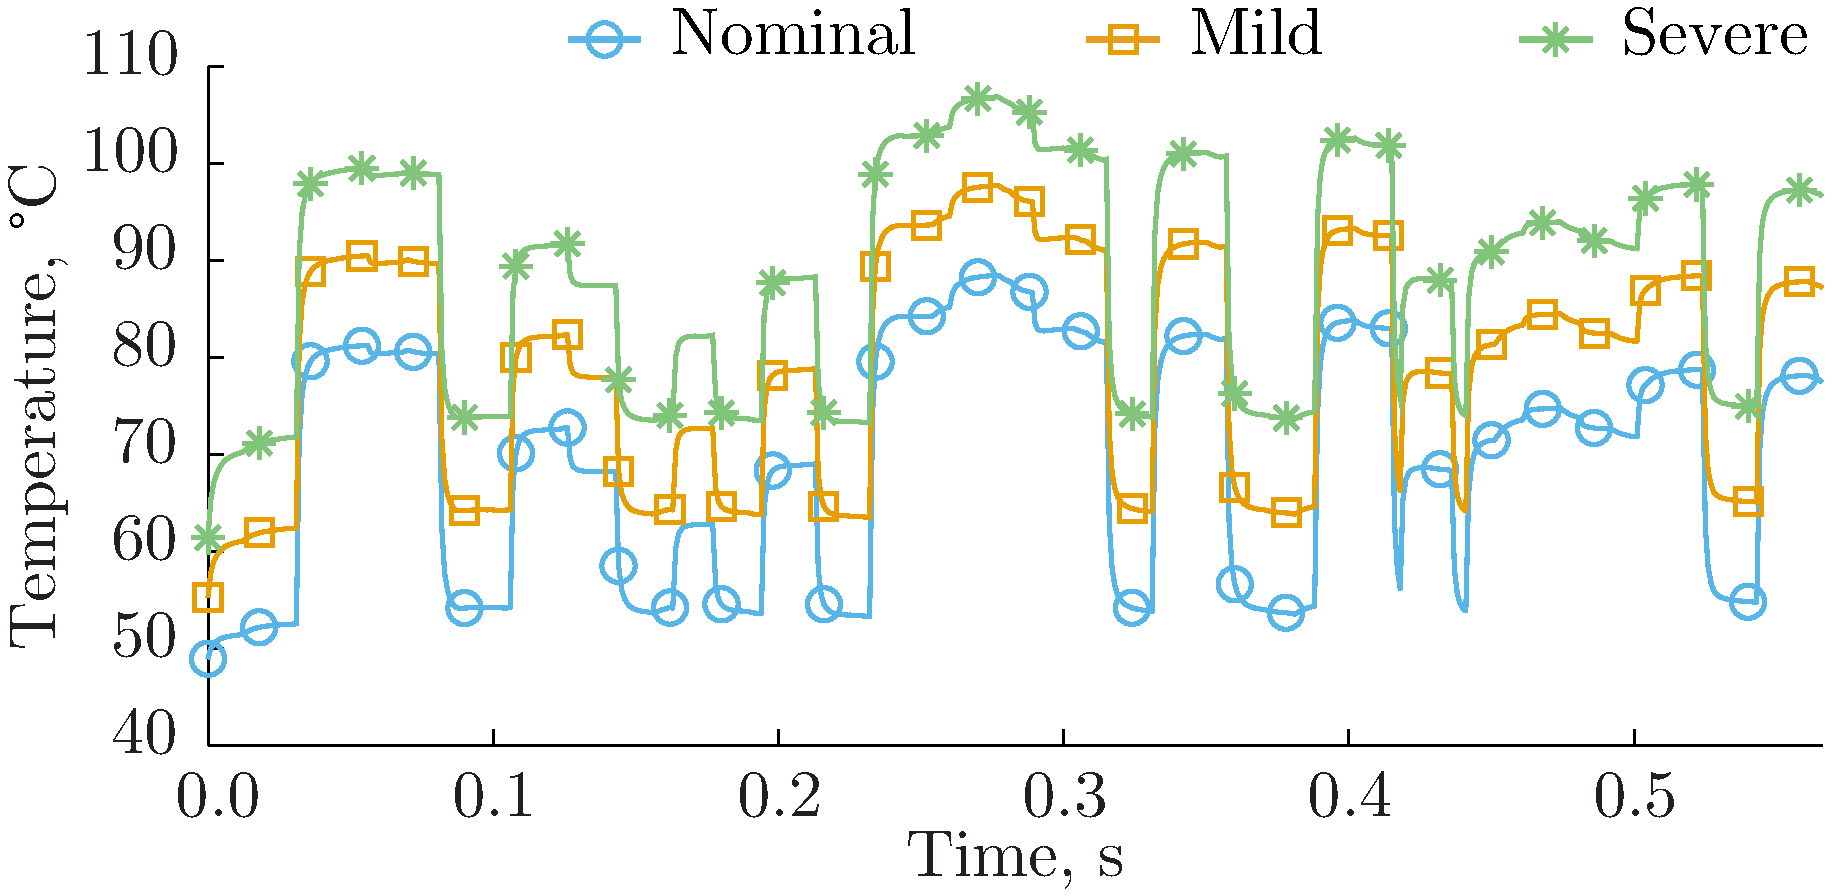
\includegraphics[width=1.0\linewidth]{include/assets/motivation-temperature.pdf}
  \vspace{-1.5em}
  \caption{Temperature fluctuation due to process variation.}
  \flabel{motivation-temperature}
\end{figure}

In order to illustrate the above concern, consider a quad-core architecture exposed to the uncertainty of the parameters that affect the leakage current.
Assume first that these parameters have nominal values.
We can then simulate the system under a certain workload and observe the corresponding temperature profile.\footnote{The experimental setup will be detailed in \sref{illustrative-example} and \sref{experimental-results}.}
The result, labeled as ``Nominal'', is depicted in \fref{motivation-temperature} where, for clarity, only one curve, corresponding to one processor, is presented (the bottom blue line). It can be seen that the temperature is always below $90^{\circ}$C.
Now let us assume a mild deviation of the parameters from the nominal values and run the simulation once again. The result is the ``Mild'' curve in \fref{motivation-temperature} (the middle orange line); the maximal temperature is approaching $100^{\circ}$C.
Finally, we repeat the experiment considering a severe deviation of the parameters and observe the curve labeled as ``Severe'' in \fref{motivation-temperature} (the top green line); the maximal temperature is almost $110^{\circ}$C.
Imagine that the designer, when tuning the solution constrained by a maximal temperature of $90^\circ$C, was guided exclusively by the nominal parameters.
In this case, even with mild deviations, the circuits might be burnt, and the amount of burnt circuits depends on the probability distribution of temperature.
Such uncertainties have to be addressed in order to pursue efficiency and fail-safeness.
Nevertheless, the majority of the literature related to power-temperature analysis of multiprocessor systems ignores this important aspect, \eg, \cite{rao2009, rai2011, thiele2011, ukhov2012}.

The remainder of the paper is organized as follows.
\sref{prior-work} provides an overview of the prior work.
In \sref{present-work}, we summarize the contribution of the present paper.
The objective of our study is formulated in \sref{problem-formulation}.
The proposed framework is presented in \sref{proposed-framework}.
A particular application of our approach is discussed in \sref{illustrative-example}, and the corresponding results are compared with MC simulations in \sref{experimental-results}.
\sref{conclusion} concludes the paper.
The work contains a set of supplementary materials with discussions on certain aspects of our framework.


  \vspace{-1.0em}
  \section{Problem Formulation} \slabel{problem-formulation} \slabel{architecture-model} \slabel{system-profiles} \slabel{preliminaries}
  \begin{figure*}
  \vspace{-1.0em}
  \centering
  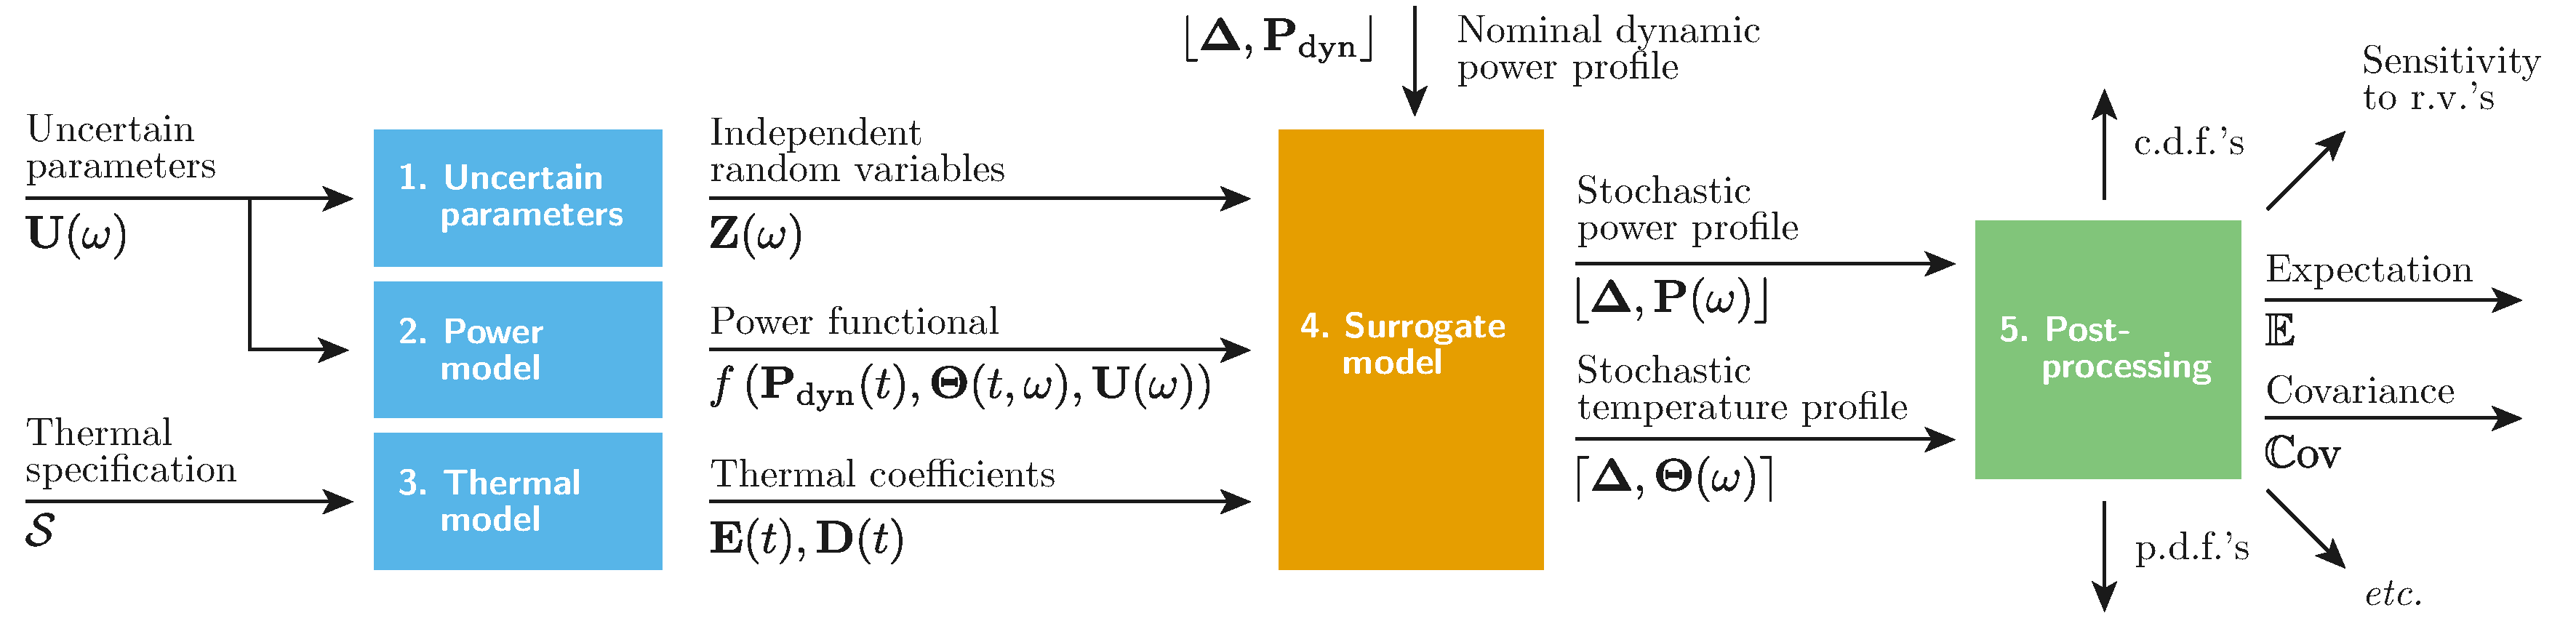
\includegraphics[width=1\textwidth]{include/assets/algorithm.pdf}
  \vspace{-1.0em}
  \caption{The structure of the proposed framework.}
  \flabel{algorithm}
  \vspace{-1.0em}
\end{figure*}

The probability space that we shall reside in is defined as a triple $(\outcomes, \sAlgebra, \pMeasure)$ where $\outcomes$ is a set of outcomes, $\sAlgebra \subseteq 2^\outcomes$ is a $\sigma$-algebra on $\outcomes$, and $\pMeasure: \sAlgebra \to [0, 1]$ is a probability measure \cite{maitre2010}.
Loosely speaking, an $n$-dimensional random variable is then a mapping $\v{X}: \o \in \outcomes \mapsto \v{X}(\o) \in \real^n$.
In what follows, the probability space $(\outcomes, \sAlgebra, \pMeasure)$ is always implied.

Consider a heterogeneous multiprocessor system that consists of $\nprocs$ processing elements and is equipped with a thermal package.
The processing elements are the active components of the system, \ie, those that dissipate power, identified at the intended level of granularity (processors, ALUs, caches, registers, \etc).
Let $\system$ be a thermal specification of the system defined as a collection of temperature-related information: (a) the floorplans of the active layers of the chip; (b) the geometry of the thermal package; and (c) the thermal parameters of the materials that the chip and package are made of.

A (transient) power profile $\profileP$ is defined as a tuple composed of a data matrix $\mP = (\vP_i) \in \real^{\nprocs \times \nsteps}$, $\vP_i \in \real^\nprocs$, that captures the power dissipation of the $\nprocs$ processing elements at $\nsteps$ moments of time and a (column) vector $\partition{\mP} = (\t_i) \in \real^{\nsteps}$ with positive and strictly increasing components that specifies these moments of time.
The definition of a (transient) temperature profile $\profileT$ is the same as the one for power except that the data matrix $\mTO$ contains temperature.

The system is assumed to depend on a set of uncertain parameters, denoted by a random vector $\vU(\o)$, $\o \in \outcomes$, which manifest themselves in deviations of the actual power dissipation from nominal values and, consequently, in deviations of temperature from the one corresponding to the nominal power consumption.
In what follows, we shall make a distinction between deterministic and stochastic profiles.
In the latter case, the power and temperature profiles are denoted by $\profileP{\o}$ and $\profileT{\o}$, respectively.

The goal of this work is to develop a probabilistic framework for power-temperature analysis (PTA) of multiprocessor systems where the actual power dissipation and temperature are stochastic due to their dependency on the set of uncertain parameters $\vU(\o)$.
The user is required to: (a) provide a thermal specification of the platform $\system$; (b) have prior knowledge (or belief) on the probability distribution of the uncertain parameters (\sref{uncertain-parameters}); and (c) specify a power model, in which $\vU(\o)$ is an input (\sref{power-model}).
The framework should provide the user with the tools to analyze the system under an arbitrary given workload and obtain the corresponding stochastic power $\profileP{\o}$ and temperature $\profileT{\o}$ profiles with a desired level of accuracy and at low costs.


  \section{Overview and Illustration}
  The basic idea of our framework is to construct a surrogate model using the theory of polynomial chaos (PC) expansions. Given such a surrogate model, quantities as cumulative distributions functions (\cdfs) and \pdfs\ can be trivially estimated. Moreover, the representations, which we compute, provide analytical formulae for probabilistic moments, \ie, the expected value, variance, \etc\ are readily available.

\subsection{Outline of the Framework} \slabel{outline}
The major steps of our technique are depicted in \fref{algorithm}:

\stage{1}{Uncertain Parameters (\sref{uncertain-parameters}).} The PC expansions operate on mutually independent \rvs. The uncertain parameters $\vU(\o)$ might not satisfy this requirement and, therefore, should be preprocessed; we shall denote the corresponding independent set of \rvs\ by $\vZ(\o)$.

\stage{2}{Power Model (\sref{power-model}).} The user specifies the power model of the system via a ``black-box'' functional $\f$, which outputs the total power $\vP(\t, \o)$ for a particular temperature $\vTO(\t, \o)$ and an outcome of the parameters $\vU(\o)$.

\stage{3}{Thermal Model (\sref{thermal-model}).} With respect to the thermal specification $\system$ defined in \sref{problem-formulation}, a mathematical model of the thermal system is constructed. The thermal model closely interacts with the power model from \stage{2}\ and produces the corresponding temperature profile.

\stage{4}{Surrogate Model (\sref{polynomial-chaos}).} The surrogate model is attained by traversing the desired time span and gradually constructing polynomial expansions, in terms of the processed uncertain parameters $\vZ(\o)$ from \stage{1}, for the stochastic power and temperature profiles. The output is essentially a substitute for the model produced at \stage{3}\ with respect to the power model determined at \stage{2}.

\stage{5}{Post-processing (\sref{output-processing}).} The computed PC expansions are analyzed in order to obtain the desired characteristics of the system, \eg, \cdfs, \pdfs, moments.


\subsection{Application to Process Variation} \slabel{application}
Before diving into details, we show a particular application of the proposed framework. Specifically, we shall perform stochastic PTA of a dual-core platform, wherein the parameters that affect the leakage current are uncertain. The application is a simplified version of the example in \sref{illustrative-example}; hence, all the omitted details will be described later on.

\begin{figure}[t]
  \vspace{-1.0em}
  \centering
  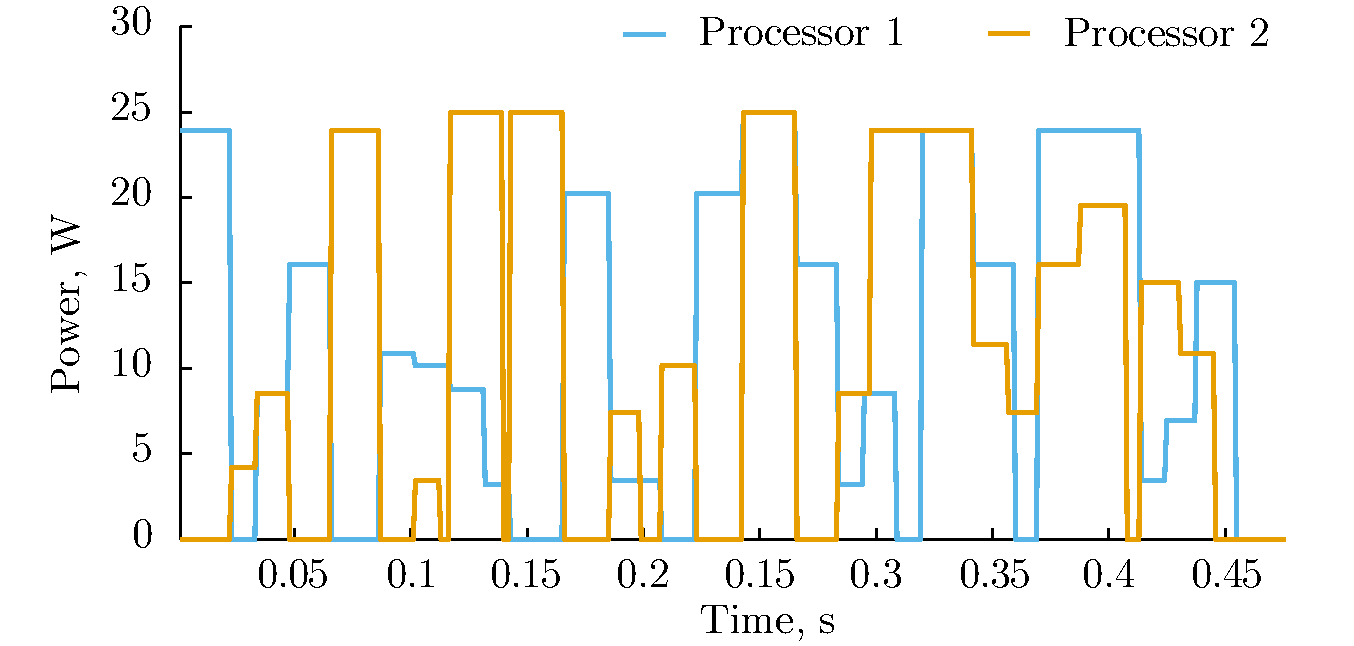
\includegraphics[width=0.90\columnwidth]{include/assets/application-power.pdf}
  \caption{A dynamic power profile.}
  \flabel{power}
  \vspace{-1.5em}
\end{figure}

\begin{figure}
  \centering
  \updatedFigure{
  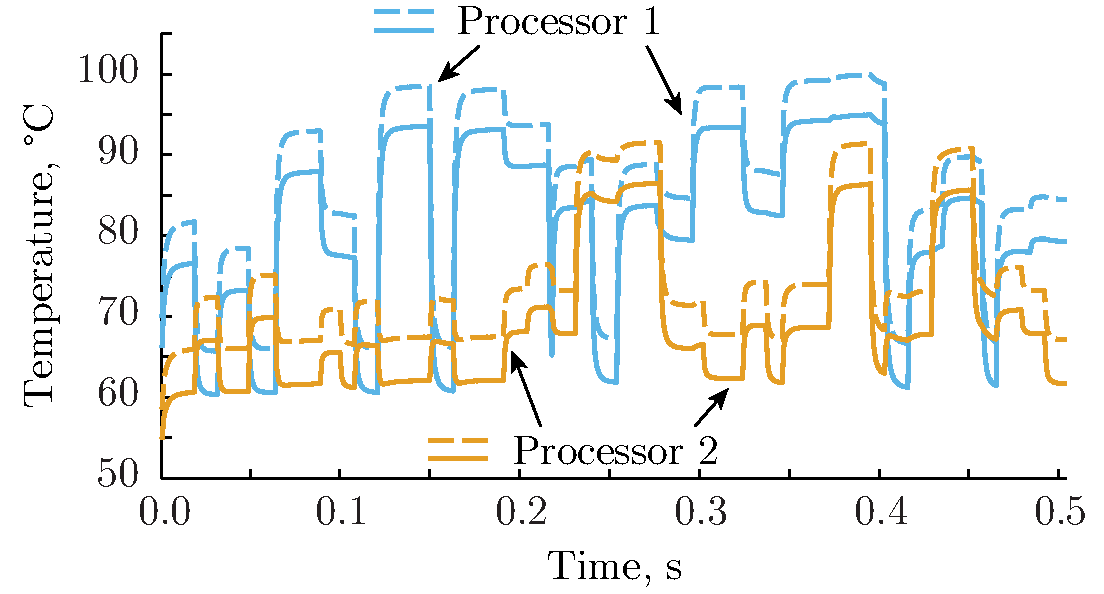
\includegraphics[width=0.90\columnwidth]{include/assets/application-temperature.pdf}
  }
  \vspace{-1.0em}
  \caption{The expected temperature (the solid lines) and one standard deviation above it (the dashed lines).}
  \flabel{application-temperature}
  \vspace{-1.0em}
\end{figure}

Without loss of generality, we address one of the most critical leakage parameters: the effective channel length \cite{chandra2010, juan2011, juan2012, srivastava2010, shen2009}. Due to process variation, the channel length is a \rv, which we denote by $\Leff(\o)$. The variations of $\Leff(\o)$ are split into global (inter-die) $\gLeff(\o)$ and local (intra-die) $\lLeff(\o)$ parts. Assume $\gLeff(\o)$ is shared among the two processors whereas each processor has its own local \rv\ $\lLeff_i(\o)$. Therefore, the channel length of the $i$th processor is
\begin{equation} \elabel{leakage-partition}
  \Leff_i(\o) = \nLeff + \gLeff(\o) + \lLeff_i(\o)
\end{equation}
where $\nLeff$ is the nominal value. Thus, the uncertain parameters, $\vU(\o)$, of the problem have been identified, \ie,
\[
  \vU(\o) = \vec{\lLeff_1(\o), \; \lLeff_2(\o), \; \gLeff(\o) }.
\]
The variations of $\Leff(\o)$ can be accurately approximated by Gaussian distributions \cite{juan2011, juan2012, srivastava2010}; hence, we assume that $\vU(\o)$ is a Gaussian vector with a given covariance matrix. Since the local \rvs\ are known to have spacial correlations, the uncertain parameters $\vU(\o)$ are not independent. Therefore, at \stage{1}\ of our framework, we transform $\vU(\o)$ into a set of independent \rvs\ denoted by $\vZ(\o) = \vec{\Z_1(\o), \; \Z_2(\o)}$, which is also Gaussian. Note, due to the correlations among $\lLeff_i(\o)$, we were also able to reduce the number of \rvs\ to two making the modeling more efficient. At \stage{2}, we decide on the power model; assume it is given as the following closed-form formula (denoted by $\f$ in \fref{algorithm}):
\begin{align*}
  & \P_i(\t, \o) = \P_{\dyn, i}(\t) + \beta_i \: \exp \left(\vphantom{\T^2_i} \alpha_0 + \alpha_1 \: \Leff_i(\o) \right. \\
  & \qquad {} + \left. \alpha_2 \: \T_i(\t, \o) + \alpha_3 \: \Leff_i(\o) \: \T_i(\t, \o) + \alpha_4 \: \T_i(\o, \t)^2 \right),
\end{align*}
for $i = 1, 2$, where $\P_{\dyn, i}(\t)$ is the dynamic power, and the rest belongs to the leakage power, which is a measurement-based model of the corresponding electrical circuits with the fitting coefficients $\alpha_j$ and $\beta_i$. Due to the separation of the dynamic and leakage parts, we only need to perform one system/power simulation of the system under the desired workload \emph{without} considering leakage and dump the corresponding nominal dynamic power profile, $\profPdyn$, of this workload; the leakage part will be added afterwards. Assume the resulting $\profPdyn$ is the one shown in \fref{application-power}. We move on to the thermal model, \stage{3}. The thermal specification $\system$ of the system at hand is assumed to be given; in particular, the floorplan of the die and the configuration of the thermal package are known. Therefore, we construct an equivalent RC thermal circuit of the system, which is depicted in \fref{circuit} in the appendix. Hence, a mathematical model of heat transfer within the platform is acquired. We transform this model in a certain way and denote the result by $\mCF(\t)$ and $\mCS(\t)$ in \fref{algorithm}. At \stage{4}, the independent \rvs, power model, and thermal model are fused together under the desired workload to produce the corresponding stochastic power $\profP{\o}$ and temperature $\profT{\o}$ profiles. The obtained stochastic profiles are nothing more than two polynomials of $\Z_1(\o)$ and $\Z_2(\o)$ with time-dependent coefficients. For example, assuming a second-total-order PC expansion, the temperature at the $k$th moment of times is
\begin{align*}
  \vTO_k(\o) &= \pccs_{k1} + \pccs_{k2} \Z_1(\o) + \pccs_{k3} \Z_2(\o) + \pccs_{k4} \Z_1(\o) \Z_2(\o) \\
  & \qquad \qquad {} + \pccs_{k5} (\Z_1(\o)^2 - 1) + \pccs_{k6} (\Z_2(\o)^2 - 1)
\end{align*}
where $\pccs_{ki}$ are vectors with two elements corresponding to the two processors. The expansion for power has the same structure but different coefficients. Such a series might be shorter or longer depending on the accuracy requirements. As we see, our surrogate model has a negligibly small computational cost to undertake UQ at \stage{5}: for any outcome of the uncertain parameters $\vZ(\o) \equiv \vZ$, we can easily compute the corresponding temperature by plugging $\vZ$ into the above equation; the same applies for power. Furthermore, the expectation and variance are calculated as simply as
\[
  \oExp{\vTO_k(\o)} = \pccs_{k1} \hspace{1em} \text{and} \hspace{1em} \oVar{\vTO_k(\o)} = \sum_{i = 2}^{6} \pcn_i \: \pccs_{ki}^2
\]
where $\pcn_i$ are normalization constants, and the squaring should be understood element-wise. For the nominal power profile $\profPdyn$ depicted in \fref{application-power}, we obtain the corresponding stochastic temperature profile $\profT{\o}$ and can observe, \eg, its expectation and standard deviation; they are plotted in \fref{application-temperature}. The displayed curves closely match those obtained via MC simulations with $10^4$ samples; however, our method takes less than a second, on a personal laptop, while the MC-based approach takes more than a day, which we shall discuss in \sref{experimental-results}. Finally, it is worth being noted that \stage{1}--\stage{2}\ are fixed for a particular platform, \ie, the corresponding outputs are tabulated and have no additional costs. In other words, various workloads of the system can be efficiently analyzed by constructing PC expansions at \stage{4}\ followed by the post-processing at \stage{5}.



  \section{Proposed Framework} \slabel{proposed-framework}
  In a nutshell, the goal stated in \sref{problem-formulation} is achieved as follows. We begin with the commonly found formalism of constructing a thermal model given a thermal specification $\system$. Due to the complexity of the underlying physical phenomenon---that is, heat transfer within a multiprocessor system---such a model is expensive from the computational perspective; this fact makes the straightforward UQ based on MC simulations prohibited and often infeasible. Instead of working directly with the obtained model, we construct a surrogate model, or a meta model, using the theory of polynomial chaos (PC) expansions. Such a representation is essentially light, \ie, the efforts needed to obtain power and temperature traces, given an outcome of the uncertain parameters, are negligible compared to those needed for the initial problem formulation. Now, the surrogate model can undergo the same sampling that one might adopt from the very beginning, but this time the procedure is undertaken in a much more efficient manner. Therefore, such quantities as \cdfs\ and \pdfs\ can be trivially estimated. Moreover, the representations, which we compute, provide analytical formulae for probabilistic moments, \ie, the expected value, variance, \etc\ are readily available without any sampling.

The major steps of our technique are depicted in \fref{algorithm} and are outlined below whereas detailed discussions are given in the following five subsections, \sref{uncertain-parameters}--\sref{output-processing}.

\step{1}{Uncertain Parameters (\sref{uncertain-parameters}).} The PC expansions, employed in this paper to perform UQ, operate on a finite set of independent \rvs. The uncertain parameters $\vU(\o)$ might not satisfy this requirement and, therefore, should be preprocessed first; the corresponding finite, independent set is denoted by $\vZ(\o)$.

\step{2}{Power Model (\sref{power-model}).} A model of the power dissipation is defined at this stage: the user determines the effect that the uncertain parameters have on the total consumption of power $\vP(\t, \o)$ given the nominal dynamic power $\vP_\dyn(\t)$, temperature $\vTO(\t, \o)$, and uncertain parameters $\vU(\o)$, for some fixed $\t$ and $\o$ (explained in \sref{uncertain-parameters}).

\step{3}{Thermal Model (\sref{thermal-model}).} With respect to the thermal specification $\system$ (see \sref{problem-formulation}), a mathematical model of the thermal system is constructed. The thermal model closely interacts with the power model from Stage~2 and produces the corresponding power and temperature profiles for a given nominal dynamic power profile and an outcome of $\vU(\o)$. As at Stage~2, the model produced at Stage~3 acts deterministically. Note that, in the context of the MC sampling, these computations would be performed thousands of times with different outcomes $\{ \vU_i \}_{i = 1}^{\mcsamples}$ of $\vU(\o)$, for some large $\mcsamples$, which, as motivated earlier, is prohibited in practice.

\step{4}{Surrogate Model (\sref{polynomial-chaos}).} The surrogate model is attained by traversing the given nominal power profile and gradually constructing polynomial expansions, in terms of the processed uncertain parameters $\vZ(\o)$ from Stage~1, for the stochastic power and temperature profiles. The output is essentially a substitute to the problem defined at Stage~3 with respect to the power model determined at Stage~2.

\step{5}{Post-processing (\sref{output-processing}).} The computed PC expansions are analyzed in order to obtain the desired characteristics of the system, \eg, \cdfs, \pdfs, moments.

\subsection{Uncertain Parameters} \slabel{uncertain-parameters}
Independence of the parameters is a prerequisite of PC expansions.
In general, however, $\vU(\o)$ can be correlated and, therefore, should be preprocessed in order to fulfill the requirement.
To this end, an adequate probability transformation should be undertaken \cite{eldred2008}.
Denote such a transformation by $\vU(\o) = \oTransform{\vZ(\o)}$, which relates the correlated uncertain parameters $\vU(\o)$ with $\nvars$ independent random variables $\vZ(\o)$.

Correlated random variables can be transformed into uncorrelated ones \via\ a linear mapping based on a factorization procedure of the covariance matrix or covariance function of $\vU(\o)$; the procedure is known as the Karhunen-Lo\`{e}ve (KL) decomposition \cite{ghanem1991}.
If, in addition, the correlated variables form a Gaussian vector then the uncorrelated ones are also mutually independent.
In the general case (non-Gaussian), the most prominent solutions to attain independence are the Rosenblatt \cite{rosenblatt1952} and Nataf transformations \cite{li2008}.\footnote{Only a few alternatives are listed here, and such techniques as independent component analysis (ICA) are left outside of the scope of the paper.}
Rosenblatt's approach is suitable when the joint probability distribution function of the uncertain parameters $\vU(\o)$ is known; however, such information is rarely available.
The marginal probability distributions and correlation matrix of $\vU(\o)$ are more likely to be given, which are already sufficient for perform the Nataf transformation.\footnote{The transformation is an approximation, which operates under the assumption that the copula of the distribution is elliptical.}
The Nataf transformation produces correlated Gaussian variables, which are then turned into independent ones by virtue of the KL decomposition mentioned earlier.

Apart from the extraction of the independent parameters $\vZ(\o)$, an essential operation at this stage is model order reduction since the number of stochastic dimensions of the problem directly impacts the complexity of the rest of the computations.
The intuition is that, due to the correlations possessed by the random variables in $\vU(\o)$, some of them can be harmlessly replaced by combinations of the rest, leading to a smaller number of the variables in $\vZ(\o)$.
This operation is often treaded as a part of the KL decomposition.

In \sref{ie-uncertain-parameters}, we shall demonstrate the Nataf transformation together with the KL decomposition.
A description of the latter can also be found in the supplementary materials, \aref{karhunen-loeve}.


\subsection{Power Model} \slabel{power-model}
In this section, we introduce the power model used in conjunction with the thermal model presented in \sref{thermal-model}. The total power dissipation of the system with $\cores$ processing elements is defined in the following abstract form:
\begin{equation} \elabel{power-model}
  \vP(\t, \o) = \f\Big(\vP_\dyn(\t), \vTO(\t, \o), \vZ(\o)\Big)
\end{equation}
where $\f: \real^\cores \times \real^\cores \times \real^\vars \to \real^\cores$ is an arbitrary function, possibly a ``black box'', of the nominal dynamic power $\vP_\dyn(\t)$, stochastic temperature $\vTO(\t, \o)$, and uncertain parameters $\vZ(\o)$. In this work, the function is assumed to be smooth in $\vZ(\o)$ and to have a finite variance, which is applicable to most physical systems \cite{xiu2002}. It can be seen that the definition of $\f$ provides a great flexibility to account for such effects as the well-known, strictly nonlinear interdependency between the leakage current and temperature \cite{srivastava2010, liu2007}. In this case, one can split the function into dynamic $\f_\dyn(\vP_\dyn(\t), \o)$ and leakage $\f_\leak(\vTO(\t, \o), \o)$ parts and define appropriate models for the components; this partition is to be further discussed in \sref{illustrative-example}.


\subsection{Thermal Model} \slabel{thermal-model}
We move on to \stage{3}\ where the thermal model of the multiprocessor system is to be established.
Given the thermal specification $\system$ of the considered platform (the floorplan of the die, the configuration of the thermal package, \etc), we employ HotSpot (v5.02) \cite{hotspot} in order to construct the equivalent thermal RC circuits of the system.
Specifically, we are interested in the coefficient matrices $\mCF(\t)$ and $\mCS(\t)$ in \eref{fourier-system} (see also \fref{algorithm}), which HotSpot helps us to compute by providing the corresponding capacitance and conductance matrices of the system as described in \aref{thermal-model}.
In this case, thermal packages are modeled with three layers, and the relation between the number of processing elements and the number of thermal nodes is given by $\nnodes = 4 \nprocs + 12$.
An example of such a circuit for a dual-core platform is depicted in \fref{circuit}.

To conclude, the power and thermal models of the platform are now acquired, and we are ready to construct the corresponding surrogate model \via\ PC expansions.


\subsection{Surrogate Model} \slabel{polynomial-chaos}
The goal is to transform the ``problematic'' term in \eref{recurrence}, \ie, the power term defined by \eref{power-model}, in such a way that the recurrence in \eref{recurrence} becomes computationally tractable. Our solution is the construction of a surrogate model for the power model in \eref{power-model}, which we further propagate through \eref{recurrence} to obtain an approximation for temperature. We employ the generalized polynomial chaos (PC) \cite{xiu2010}, which decomposes stochastic quantities into infinite series of orthogonal polynomials of \rvs. Such a series is especially attractive from the post-processing perspective as it is nothing more than a polynomial, hence, easy to interpret and evaluate. An introduction to orthogonal polynomials is given in \aref{orthogonal-polynomials}.

The first step towards a PC expansion is the choice of a suitable polynomial basis $\{ \pcb_i(\vz) \}$, which is typically picked from the Askey scheme of orthogonal polynomials \cite{xiu2010}. The step is crucial as the rate of convergence of PC expansions closely depends on it. There are no strict rules that guarantee the optimal choice \cite{maitre2010, knio2006}; however, there are best practices which say that one should be guided by the probability distributions of the \rvs\ that drive the stochastic system (see \aref{polynomial-chaos}). \tref{askey} in the appendix displays several examples of such paired probability distributions and polynomial bases. For instance, when the \rvs\ $\vZ(\o)$ follow a beta distribution, the Jacobi basis is worth being tried first. On the other hand, the Hermite basis (\fref{hermite}) is preferable for Gaussian \rvs.

Having an appropriate basis chosen, we apply the PC procedure to power in \eref{recurrence} and truncate the resulting infinite series in order to make it feasible for practical implementations. Such an expansion is formally defined as
\begin{equation} \elabel{pc-expansion}
  \oPC{\vars}{\pcorder}{\vP_k(\o)} = \sum_{i = 1}^{\pcterms} \pcc{\vP}_{ki} \; \pcb_i(\vZ(\o))
\end{equation}
where $\{ \pcb_i(\vZ(\o)) \}_{i = 1}^{\pcterms}$ is the truncated basis with $\pcterms$ polynomial terms of $\vars$ variables, and $\pcc{\vP}_{ki} \in \real^\cores$ are the coefficients of the expansion. The latter are computed using spectral projections as it is explained in the appendix, \aref{spectral-projection}. $\pcorder$ denotes the order of the expansion, which determines the maximal degree of the $\vars$-variate polynomials involved in the expansion; hence, $\pcorder$ also defines accuracy.

It can be seen in \eref{recurrence} that, due to the linearity of the operations involved in the recurrence, $\vX_k(\o)$ retains the same polynomial structure as $\vP_k(\o)$. Therefore, using \eref{pc-expansion}, \eref{recurrence} is rewritten as follows, for $k = 1, \dotsc, \steps$:
\begin{equation} \elabel{expanded-recurrence}
  \oPC{\vars}{\pcorder}{\vX_k(\o)} = \mCF_k \: \oPC{\vars}{\pcorder}{\vX_{k-1}(\o)} + \mCS_k \: \oPC{\vars}{\pcorder}{\vP_k(\o)}.
\end{equation}
Thus, there are two PC expansions for two concurrent stochastic processes with the same basis but different coefficients. As shown in \aref{spectral-projection}, \eref{expanded-recurrence} can be reduced to
\begin{equation} \elabel{pc-recurrence}
  \pcc{\vX}_{ki} = \mCF_k \: \pcc{\vX}_{(k - 1)i} + \mCS_k \: \pcc{\vP}_{ki}
\end{equation}
where $k = 1, \dotsc, \steps$ and $i = 1, \dotsc, \pcterms$. Finally, \eref{fourier-output} and \eref{pc-recurrence} are combined together to compute the coefficients of the PC expansion of the temperature vector $\vTO_k(\o)$.

To summarize, let us recall the stochastic recurrence in \eref{recurrence} where, in the presence of correlations, an arbitrary functional $\vP_k(\omega)$ of the uncertain parameters $\vU(\o)$ and random temperature $\vTO_k(\o)$ (see \sref{power-model}) needs to be evaluated and combined with another random vector, $\vX_k(\omega)$. Now, the recurrence in \eref{recurrence} has been replaced with a purely deterministic recurrence in \eref{pc-recurrence} that involves only linear operations. Moreover, the performed spectral decompositions have substituted the heavy thermal system in \eref{fourier-system} with a light polynomial surrogate defined by a set of basis functions $\{ \pcb_i(\vz) \}$ and the corresponding sets of coefficients, namely, $\{ \pcc{\vP}_{ki} \}$ for power and $\{ \pcc{\vTO}_{ki} \}$ for temperature, where $k$ traverses all the $\steps$ intervals $\dt_k$ of the considered time span. Consequently, the output of the proposed framework constitutes two stochastic profiles, the power $\profP{\o}$ and temperature $\profT{\o}$ profiles, that are ready to be analyzed from the UQ perspective.


\subsection{Post-processing} \slabel{output-processing}
Due to the properties of PC expansions, specifically, due to the basis functions and their pairwise orthogonality (see \aref{orthogonal-polynomials}), the obtained polynomial traces are trivial for various prospective analyses. For instance, consider the PC expansion of temperature at the $k$th time interval given as
\vspace{-0.2em}%
\begin{equation} \elabel{pc-k}
  \oPC{\vars}{\pcorder}{\vTO_k(\o)} = \sum_{i = 1}^{\pcterms} \pcc{\vTO}_{ki} \pcb_i(\vZ(\o))
\end{equation}
\vspace{-0.2em}%
where $\pcc{\vTO}_{ki}$ are computed using \eref{fourier-output} and \eref{pc-recurrence}. Let us, for example, find the expectation and variance of the expansion. As shown in \aref{spectral-projection}, these values have the following simple expressions solely based on the coefficients:
\vspace{-0.2em}%
\begin{equation} \elabel{pc-moments}
  \oExp{\vTO_k(\o)} = \pcc{\vTO}_{k1} \hspace{1em} \text{and} \hspace{1em} \oVar{\vTO_k(\o)} = \sum_{i = 2}^{\pcterms} \pcn_i \: \pcc{\vTO}_{ki}^2
\end{equation}
\vspace{-0.2em}%
for expectation and variance, respectively, where the squaring is element-wise, and $\pcn_i$ are normalization constants with analytical expressions. Such quantities as \cdfs\ and \pdfs\ can be estimated by sampling \eref{pc-k}; each sample is a trivial evaluation of a polynomial. Furthermore, global and local sensitivity analyses of deterministic and non-deterministic quantities can be readily conducted on \eref{pc-k}.



  \section{Illustrative Example} \slabel{illustrative-example}
  In this section, we demonstrate the proposed framework applying it to leakage power and temperature analysis under process variation.

\subsection{Problem Identification} \slabel{ie-problem-formulation}
The power dissipation is composed of two major parts: dynamic and leakage. The influence of the process variation on the dynamic power is known to be negligibly small \cite{juan2011, juan2012, srivastava2010}; on the other hand, the variability of leakage is substantial, in which the subthreshold current contributes the most \cite{juan2011, juan2012}. Hence, we focus on the subthreshold leakage and, more specifically, on the effective channel length $\Leff$. The variations of $\Leff$ are split into global (inter-die) and local (intra-die) parts \cite{chandra2010, juan2011, juan2012, srivastava2010, shen2009}. The global offset is shared among all the processing elements, i.e., it is a single \rv, whereas there are $\cores$ distinct \rvs\ for the local deviations. Therefore, the channel length within the $i$th processing element is given as
\[
  \Leff_i(\o) = \nLeff + \gLeff(\o) + \lLeff_i(\o)
\]
where $\nLeff$ is the nominal channel length, $\gLeff(\o)$ is a zero-mean \rv\ that represents the global variation, and $\lLeff_i(\o)$ is a zero-mean \rv\ for the local component. Consequently, the uncertain parameters of the current model are $\vU(\o) = \vec{\lLeff_1(\o), \dotsc, \lLeff_\cores(\o), \gLeff(\o) }$. The global \rv\ is typically assumed to be uncorrelated with respect to the local ones while the latter are known to be highly correlated among each other. Without loss of generality, we employ the following radial model of correlation for $\lLeff_i(\o)$ \cite{ghanem1991, cheng2011}:
\begin{equation} \elabel{correlation-matrix}
  \oCorr{\lLeff_i(\o), \lLeff_j(\o)} = e^{-|r_i - r_j|/\corrLength}
\end{equation}
where $r_i$ is the distance between the $i$th processing element and the center of the die, and $\corrLength$ is the correlation length. For convenience, the resulting correlation matrix is extended by one dimension to pack $\gLeff(\o)$ and $\lLeff_i(\o)$ together. In this case, the matrix obtains one additional non-zero element on the diagonal. Taking into account the variances of the \rvs, the covariance matrix denoted by $\mCov_\vU$ is formed.


\subsection{Uncertain Parameters Processing} \slabel{ie-uncertain-parameters}
As mentioned in \sref{uncertain-parameters}, $\vU(\o)$ should be preprocessed to extract a set of mutually independent \rvs, $\vZ(\o)$. It is generally accepted that the variations of the channel length are distributed normally \cite{juan2011, juan2012, srivastava2010}, i.e., $\vU(\o) \sim \normal{\vZero}{\mCov_\vU}$; therefore, an appropriate linear transformation can be employed. More specifically, the procedure described in this section is known as the principal component analysis (PCA), which is the finite-dimensional version of the KL expansion.

Since any covariance matrix is necessarily a real, symmetric matrix, it admits the eigenvalue factorization \cite{press2007} as $\mCov_\vU = \m{V} \m{\Lambda} \m{V}^T$ where $\m{V}$ and $\m{\Lambda}$ are an orthogonal matrix of the eigenvectors and a diagonal matrix of the eigenvalues of $\mCov_\vU$, respectively. Consequently, $\vU(\o)$ can be decomposed as $\vU(\o) = \m{V} \m{\Lambda}^\ifrac{1}{2} \vZ(\o) = \oInvTransform{\vZ(\o)}$ where $\vZ(\o) \sim \normal{\vZero}{\mI}$ is the desired vector of centered, normalized, and mutually independent uncertain parameters, and $\oInvTransform{\idot}$ is the corresponding inverse transformation (see \sref{uncertain-parameters}).

The number of stochastic dimensions $\vars$, which so far is $\cores + 1$, directly impacts the computational cost of a PC expansion as it is seen in \eref{pc-terms}. Therefore, one should consider a possibility of model order reduction before constructing PC expansions. The intuition is that, due to the existing correlations between \rvs, some of them can be harmlessly replaced by linear combinations of the rest. One way to reveal these redundancies is to analyze the eigenvalues $\lambda_i$ found in $\m{\Lambda}$. Assume $\lambda_i$, $\forall i$, are arranged in a non-increasing order and let $\bar{\lambda}_i = \lambda_i / \sum_j \lambda_j$. Gradually summing up the arranged and normalized eigenvalues $\bar{\lambda}_i$, we can identify a subset of them, which has the cumulative sum greater than a certain threshold $\Lth$. When $\Lth$ is sufficiently high (close to 1), the rest of the eigenvalues and their eigenvectors can be dropped as being insignificant, reducing the number of stochastic dimensions $\vars$. The results of the algorithm are reported in \sref{experimental-results}.


\subsection{Power and Thermal Models Construction} \slabel{ie-power-model}
At this stage, we need to construct a leakage model with the identified uncertain parameters $\vU(\o)$ and temperature as inputs. To this end, \eref{power-model} is decomposed into the sum of dynamic and leakage components denoted respectively by $\f_\dyn(\vP_\dyn(\t), \o)$ and $\f_\leak(\vTO(\t, \o), \o)$. As motivated in \sref{ie-problem-formulation}, we let $\f_\dyn(\vP_\dyn(\t), \o) = \vP_\dyn(\t)$. A model for the other part, i.e., the leakage power, can be obtained by, for instance, a set of SPICE-type simulations of reference electrical circuits. In our example, we employ a circuit based on the Predictive Technology Model \cite{ptm}. A surface fitting procedure is then carried out on the output data, and the following exponential model is acquired:
\begin{equation} \elabel{leakage-current}
  I_\leak(\Leff, \T) = \text{exp} \big\{ \alpha_0 + \alpha_1 \Leff + \alpha_2 \T + \alpha_3 \Leff \T + \alpha_4 \T^2 \big\}
\end{equation}
where $\alpha_i$ are fitting coefficients. The reference leakage current $I_\leak(\Leff, \T)$ is further scaled up to the power level of each of the processing elements. Finally, we have
\[
  \f_{\leak, i}(\T_i(\t, \o), \o) = \beta_i I_{\leak, i}(\Leff_i(\o), \T_i(\t, \o))
\]
for $i \in \{ 1, \dotsc, \cores \}$ where $\beta_i$ are scaling coefficients.

In order to construct equivalent thermal RC circuits, we first utilize HotSpot v5.02 \cite{hotspot} in order to obtain the thermal capacitance $\mC$ and conductance $\mG$ matrices. In this case, thermal packages are modeled with three layers, and the relation between the number of processing elements and the number of thermal nodes is $\nodes = 4 \cores + 12$. Then, we use the technique described in \cite{ukhov2012} to compute the coefficient matrices $\mE(\t)$ and $\mD(\t)$ of the recurrence in \eref{recurrence}.


\subsection{Polynomial Chaos Expansion} \slabel{ie-polynomial-chaos}
In the current scenario, the PC is to be founded on the Hermite polynomial basis as it is optimal for $\vZ(\o) \sim \normal{\vZero}{\mI}$ \cite{xiu2002}. To illustrate the basis, in the two-dimensional case, the first Hermite polynomials $\pcb_i(\{ \Z_1(\o), \Z_2(\o) \})$ are
\[
  \begin{array}{lllllll}
  1, & \Z_1, & \Z_2, & \Z_1^2 - 1, & \Z_1 \Z_2, & \Z_2^2 - 1, & \dotsc
  \end{array}
\]
The PC coefficients in \eref{pc-expansion} should be evaluated according to the multidimensional integral in \eref{inner-product-integral}. In numerical integration, this task is accomplished by virtue of a quadrature rule \cite{press2007}. Since we need to compute expectations with respect to normal measures, the Gauss-Hermite quadrature rule is of a particular interest. The rule is a Gaussian rule; therefore, the order $\qdorder$, i.e., the number of integration points involved, and precision $\qdprecision$, i.e., the maximal total order of polynomials that the rule integrate exactly, are related as $\qdprecision = 2 \qdorder - 1$, which makes such quadratures especially efficient \cite{heiss2008}. Using the family of the one-dimensional Gauss-Hermite rules, a multivariate quadrature is constructed. In low dimensions, the construction is based on the direct tensor produce of the one-dimensional rules; however, in high dimensions, the number of points computed by this technique can easily explode. To overcome the problem, we employ the Smolyak algorithm, which preserves the accuracy of the underlying one-dimensional rules for complete polynomials while significantly reducing the number of integration points \cite{eldred2009, maitre2010, heiss2008}. The $\vars$-variate quadrature rule of level $\qdlevel$ is defined as
\[
  \oQuad{\vars}{\qdlevel}{f} \eqdef \sum_{i = 1}^{\qdorder} f(\qdn{\vZ}_i) \qdw_i
\]
where $\qdn{\vZ}_i \in \real^\vars$ and $\qdw_i \in \real$ are the prescribed integration points and their weights, respectively. The level $\qdlevel$ is defined as the index of the quadrature in the corresponding family of rules with increasing precision; this value should be chosen in such a way that the rule is exact for polynomials of total order at least $2 \pcorder$ (twice the order of the PC expansion), which can be seen in \eref{pc-coefficients} \cite{eldred2009}. Therefore, $\qdlevel \geq \pcorder + 1$ since the quadrature is Gaussian. Hence, \eref{pc-coefficients} is rewritten as
\[
  \pcc{\vP}_i(0) = \frac{1}{\pcn_i} \oQuad{\vars}{\qdlevel}{\vP(0, \o) \pcb_i(\vZ(\o))}
\]
where $\{ \pcn_i \}_{i = 1}^{\pcterms}$ are computed exactly either by directly using the same quadrature rule or by taking products of one-dimensional counterparts with known analytical expressions \cite{xiu2010}; the result is further tabulated.

At this point, we have completed four out of five steps of the proposed framework depicted in \fref{algorithm}. As a result, at each moment of time, we have two vector-valued polynomials, one for power and one for temperature, defined in terms of RVs; an example of such a polynomial is given in \eref{pc-k}. Now, the polynomials can be trivially analyzed to retrieve the needed characteristics of the system, and this is the fifth step in \fref{algorithm}, which we shall discuss in the following section.



  \section{Experimental Results} \slabel{experimental-results}
  In this section, numerical results of the proposed UQ framework for the illustrative example in \sref{illustrative-example} are reported.\footnote{All the experiments are implemented in MATLAB R2012b \cite{matlab} and conducted on a GNU/Linux machine with Intel Core i7 3.4~GHz and 8~GB of RAM.}

The channel length $\Leff$ is assumed to deviate by $5\%$ from the nominal value of 45 nm where the global and local variations are equally weighted \cite{juan2011, juan2012}. The \rvs\ that represent the intra-die variability are computed by the KL expansion applied to \eref{covariance-function} (see \aref{uncertain-parameters}), wherein the correlation length $\corrLength$ is half the size of the die. Dynamic power profiles involved in the experiments are based on simulations of randomly generated applications constructed as directed acyclic task graphs.\footnote{The task graphs of the applications, floorplans of the platforms, configuration of HotSpot, which is used to construct the thermal RC circuits, are available online at \cite{sources}.} The floorplans of the platforms are constructed in such a way that the processing elements form regular grids, as it is the case with, \eg, Alpha 21264 studied in \cite{juan2011}. Time steps of power and temperature traces are set to one millisecond, \ie, $\dt_i = 10^{-3}$~s (see \sref{problem-formulation}). The reference leakage current $I_\leak(\Leff, \T)$ (see \sref{ie-power-model}) is scaled such that the leakage power accounts for about $40\%$ of the total power at high temperatures \cite{liu2007}. To assess the performance of our framework, we employ a Monte Carlo (MC) sampling technique. For each sample draw, the MC approach solves the initial problem numerically using the Dormand-Prince method provided by MATLAB; the procedure combines the well-known fourth- and fifth-order Runge-Kutta formulas \cite{press2007}. Based on theoretical estimations \cite{diaz-emparanza2002} of the MC accuracy, experience from the literature \cite{xiu2010, eldred2009, maitre2010, shen2009}, and our observations, we let the MC approach with a rather moderate number of $10^4$ samples be the etalon for the evaluation of the proposed technique.

The first set of experiments is aimed to identify the accuracy of our framework with respect to MC simulations.
At this point, it is important to note that the true distributions of temperature are unknown, and both the PC and MC approaches introduce errors.
These errors decrease as the order of PC expansions, $\pcorder$, and the number of MC samples, $\nsamples$, respectively, increase.
Therefore, instead of postulating that the MC technique with a certain number of samples is the ``universal truth'' that we should achieve, we shall vary both $\pcorder$ and $\nsamples$ and monitor the corresponding difference between the results produced by the two alternatives.

In order to make the comparison even more comprehensive, let us also inspect the effect of the correlation patterns between the local random variables $\lLeff_i(\o)$ (recall \sref{illustrative-example}).
Specifically, apart from $\pcorder$ and $\nsamples$, we shall change the balance between the two correlation kernels shown in \eref{correlation-function}, \ie, the squared-exponential $\fCorr_\SE$ and Ornstein-Uhlenbeck $\fCorr_\OU$ kernels, which is controlled by the weight parameter $\eta \in [0, 1]$.
In reality, of course, this parameter can take any value between zero and one.
Consequently, prior to any analysis, it should be determined based on the knowledge of the correlation structures typical for the fabrication process utilized.

The PC and MC methods are compared by means of three error metrics.
The first two are the normalized root mean square errors (\nrmses) of the expectation and variance of the computed temperature profiles.\footnote{In the context of \nrmses, we treat the MC results as the observed data and the PC results as the corresponding model predictions.}
The third metric is the mean of the \nrmses\ of the empirical \pdfs\ of temperature constructed at each time step for each processing element.
The metrics are denoted by $\eExp$, $\eVar$, and $\ePDF$, respectively.
$\eExp$ and $\eVar$ are easy to interpret, and they are based on the analytical formulae in \eref{pc-moments}.
$\ePDF$ is a strong indicator of the quality of the distributions estimated by our framework, and it is computed by sampling the constructed PC expansions.
In contrast with the MC approach, this sampling has a negligible overhead as we discussed in \sref{post-processing}.

The considered values for $\pcorder$, $\nsamples$, and $\eta$ are the sets $\{ n \}_{n = 1}^7$, $\{ 10^n \}_{n = 2}^5$, and $\{ 0, 0.5, 1 \}$, respectively.
The three cases of $\eta$ correspond to the total dominance of $\fCorr_\OU$ ($\eta = 0$), perfect balance between $\fCorr_\SE$ and $\fCorr_\OU$ ($\eta = 0.5$), and total dominance of $\fCorr_\SE$ ($\eta = 1$).
A comparison for a quad-core architecture with a dynamic power profile of $\nsteps = 10^2$ steps is given in \tref{accuracy-eta-0}, \tref{accuracy-eta-0-5}, and \tref{accuracy-eta-1}, which correspond to $\eta = 0$, $\eta = 0.5$, and $\eta = 1$, respectively.
Each table contains three subtables: one for $\eExp$ (the left most), one for $\eVar$ (in the middle), and one for $\ePDF$ (the right most), which gives nine subtables in total.
The columns of the tables that correspond to high values of $\nsamples$ can be used to assess the accuracy of the constructed PC expansions; likewise, the rows that correspond to high values of $\pcorder$ can be used to judge about the sufficiency of the number of MC samples.
One can immediately note that, in all the subtables, all the error metrics tend to decrease from the top left corners (low values of $\pcorder$ and $\nsamples$) to the bottom right corners (high values of $\pcorder$ and $\nsamples$), which suggests that the PC and MC methods converge.
There are a few outliers, associated with low PC orders and/or the random nature of sampling, \eg, $\eVar$ increases from 66.13 to 66.70 and $\ePDF$ from 1.59 to 1.62 when $\nsamples$ increases from $10^4$ and $10^5$ in \tref{accuracy-eta-0-5}; however, the aforementioned main trend is still clear.

For clarity of the discussions below, we shall primarily focus on one of the tables, namely, on the middle table, \tref{accuracy-eta-0-5}, as the case with $\eta = 0.5$ turned out to be the most challenging (explained in \sref{er-speed}).
The drawn conclusions will be generalized to the other two tables later on.

In this section, we focus on the computational speed of our framework.
First, we vary the number of processing elements $\nprocs$, which directly affects the dimensionality of the uncertain parameters $\vU(\o) \in \real^{\nprocs + 1}$ (recall \sref{illustrative-example}).
As before, we shall report the results obtained for various correlation weights $\eta$, which impacts the number of the independent variables $\vZ(\o) \in \real^\nvars$, preserved after the KL-based model order reduction procedure described in \sref{ie-uncertain-parameters} and \aref{karhunen-loeve}.

The results including the dimensionality of $\vZ(\o)$, $\nvars$, are given in \tref{speed-processing-elements} where the considered values for $\nprocs$ are $\{ 2^n \}_{n = 1}^5$, and the number of time steps $\nsteps$ is set to $10^3$.
It can be seen that the correlation patters inherent to the fabrication process \cite{cheng2011} open a great possibility for model order reduction: $\nvars$ is observed to be at most 12 while the maximal number without reduction is 33 (one global variable and 32 local ones corresponding to the case with 32 processing elements).
One can also observe how this number changes with respect to $\eta$: on average, the $\fCorr_\OU$ kernel ($\eta = 0$) requires the fewest number of variables while the mixture of $\fCorr_\SE$ and $\fCorr_\OU$ ($\eta = 0.5$) requires the most.\footnote{The results in \sref{er-accuracy} correspond to the case with $\nprocs = 4$; therefore, $\nvars$ is two, five, and five for \tref{accuracy-eta-0}, \tref{accuracy-eta-0-5}, and \tref{accuracy-eta-1}, respectively.}
It means that, in the latter case, more variables should be preserved in order to retain 99\% of the variance of the data; hence, the case with $\eta = 0.5$ is the most demanding in terms of complexity (see \sref{computational-challenges}).

Another observation, found in \tref{speed-processing-elements}, is the low slope of the execution time of the MC technique, which illustrates the well-known fact that the workload per one MC sample is independent of the number of stochastic dimensions \cite{maitre2010}.
On the other hand, the rows with $\nvars > 10$ hint at the curse of dimensionality possessed by PC expansions, which was discussed in \sref{computational-challenges}.
However, even in high dimensions, the proposed framework significantly outperforms MC sampling. For instance, in order to analyze a power profile with $10^3$ steps of a system with 32 cores, the MC approach requires more than 40 hours whereas the proposed framework takes less than two minutes (the case with $\eta = 0.5$).

Finally, we investigate the scaling properties of the proposed framework with respect to the duration of the considered time spans, which is directly proportional to the number of steps $\nsteps$ in the power and temperature profiles.
The results for a quad-core architecture are given in \tref{speed-time-spans}.
Due to the long execution times demonstrated by the MC approach, its statistics for high values of $\nsteps$ are extrapolated based on a smaller number of samples, \ie, $\nsamples \ll 10^4$.
As it was noted before regarding the results in \tref{speed-processing-elements}, we observe the dependency of the PC expansions on the dimensionality of $\vZ(\o)$, $\nvars$, which is two for $\eta = 0$ and five for the other two values of $\eta$ (see \tref{speed-processing-elements} for $\nprocs = 4$).
It can be seen in \tref{speed-time-spans} that the computational times of both methods grow linearly with $\nsteps$, which is expected.
However, the proposed framework shows a vastly superior performance being five orders of magnitude faster than MC sampling.

\begin{figure}[b]
  \vspace{-1.5em}
  \centering
  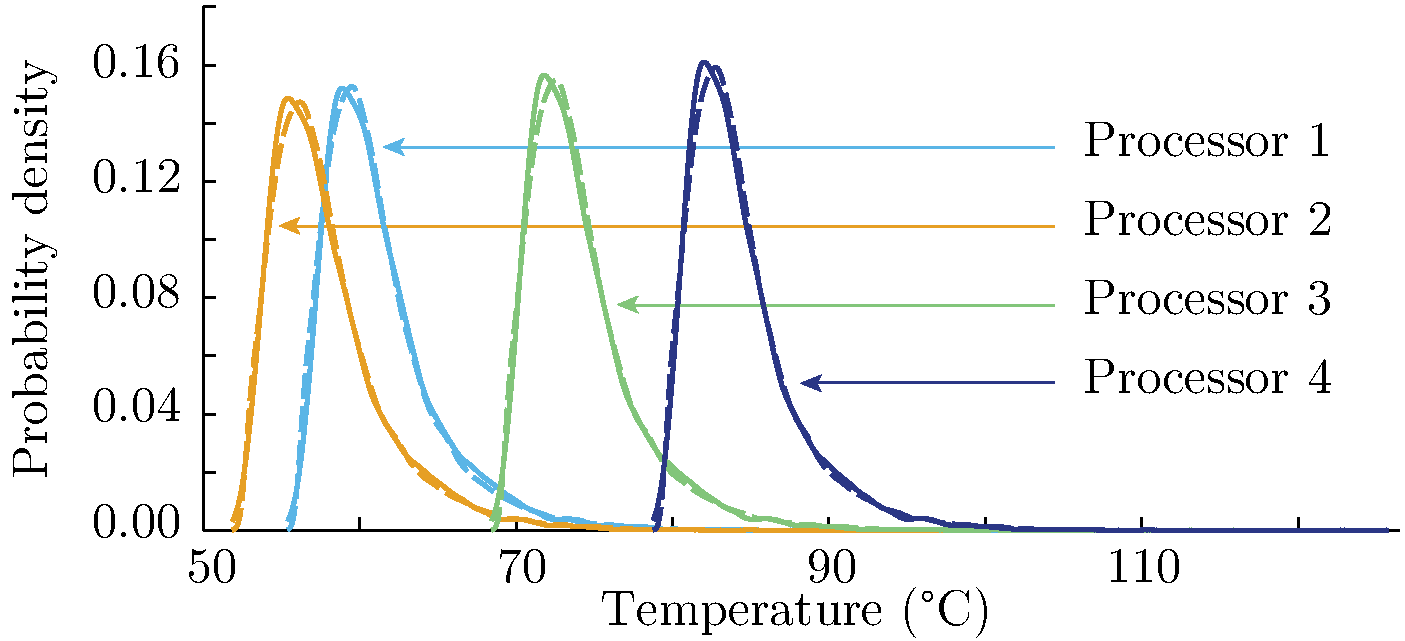
\includegraphics[width=1\ColumnWidth]{include/assets/experimental-results-pdf.pdf}
  \vspace{-2.0em}
  \caption{Probability density functions computed at time 50$\,\text{ms}$ using the proposed framework (the dashed lines) and MC sampling (the solid lines).}
  \flabel{experimental-results-pdf}
\end{figure}

First, we concentrate on the accuracy of our technique and, thus, pay particular attention the columns of \tref{accuracy-eta-0-5} corresponding to high values of $\nsamples$.
It can be seen that the error of the expected value, $\eExp$, is small even for $\pcorder = 1$: it is bounded by 0.6\% (see $\eExp$ for $\pcorder \geq 1$ and $\nsamples \geq 10^4$).

The error of the second central moment, $\eVar$, starts from 66.7\% for the first-order PC expansions and drops significantly to 5.71\% and below for the fourth order and higher (see $\eVar$ for $\pcorder \geq 4$ and $\nsamples = 10^5$).
It should be noted, however, that, for a fixed $\pcorder \geq 4$, $\eVar$ exhibits a considerable decrease even when $\nsamples$ transitions from $10^4$ to $10^5$.
The rate of this decrease suggests that $\nsamples = 10^4$ is not sufficient to reach the same accuracy as the one delivered by the proposed framework, and $\nsamples = 10^5$ might not be either.

The results of the third metric, $\ePDF$, allow us to conclude that the \pdfs\ computed by the third-order (and higher) PC expansions closely follow those estimated by the MC technique with large numbers of samples, namely, the observed difference in \tref{accuracy-eta-0-5} is bounded by 1.83\% (see $\ePDF$ for $\pcorder \geq 3$ and $\nsamples \geq 10^4$).
To give a better appreciation of the proximity of the two methods, \fref{experimental-results-pdf} displays the \pdfs\ computed using our framework for time moment 50~ms with $\pcorder = 4$ (the dashed lines) along with those calculated by the MC approach with $\nsamples = 10^4$ (the solid lines).
It can be seen that the \pdfs\ tightly match each other.
Note that this example captures one particular time moment, and such curves are readily available for all the other steps of the considered time span.

Now we take a closer look at the convergence of the MC-based technique.
With this in mind, we focus on the rows of \tref{accuracy-eta-0-5} that correspond to PC expansions of high orders.
Similar to the previous observations, even for low values of $\nsamples$, the error of the expected values estimated by MC sampling is relatively small, namely, bounded by 1.19\% (see $\eExp$ for $\pcorder \geq 4$ and $\nsamples = 10^2$).
Meanwhile, the case with $\nsamples = 10^2$ has a high error rate in terms of $\eVar$ and $\ePDF$: it is above 38\% for variance and almost 3.5\% for \pdfs\ (see $\eVar$ and $\ePDF$ for $\pcorder = 7$ and $\nsamples = 10^2$).
The results with $\nsamples = 10^3$ are reasonably more accurate; however, this trend is compromised by \tref{accuracy-eta-1}: $10^3$ samples leave an error of more than 7\% for variance (see $\eVar$ for $\pcorder \geq 4$ and $\nsamples = 10^3$).

The aforementioned conclusions, based on \tref{accuracy-eta-0-5} ($\eta = 0.5$), are directly applicable to \tref{accuracy-eta-0} ($\eta = 0$) and \tref{accuracy-eta-1} ($\eta = 1$).
The only difference is that the average error rates are lower when either of the two correlation kernels dominates.
In particular, according to $\eVar$, the case with $\eta = 1$, which corresponds to $\fCorr_\SE$, stands out to be the least error prone.

Guided by the observations in this subsection, we conclude that our framework delivers accurate results starting from $\pcorder = 4$.
The MC estimates, on the other hand, can be considered as sufficiently reliable starting from $\nsamples = 10^4$.
The last conclusion, however, is biased in favor of the MC technique since, as we noted earlier, there is evidence that $10^4$ samples might still not be enough.

The first set of experiments is aimed to identify the accuracy of our framework and, consequently, to find a reasonable value of the polynomial order $\pcorder$ (see \sref{polynomial-chaos}). To this end, three accuracy metrics have been chosen. The first two are the normalized root mean square errors (\nrmse) of expectation and variance of the resulting temperature traces. The third metric is the mean of \nrmses\ of empirical \pdfs\ constructed at each time step for each processing element. The comparison for a quad-core architecture with a dynamic power profile of $\steps = 10^2$ steps is given in \fref{accuracy}, where $\pcorder$ is swept from one to seven. It can be seen that deviations of expectation is small even for $\pcorder = 1$ and is bounded by $1\%$. The \nrmse\ of variance starts from $38\%$ for the first-order PC expansion and drops significantly to less than $5\%$ for the fifth-order PC. The result of the third error estimate, the \nrmse\ of \pdfs, is of particular importance since it allows us to conclude that the \pdfs\ computed by the third-order (and higher) PC expansions are closely following those of the MC technique with a large number of samples. Guided by the above observations, we fix the polynomial order $\pcorder$ to five for the rest of the experiments and state that the error of our technique is bounded by less than $0.5\%$ for expectations, less than $5\%$ for variances, and less than $2\%$ for \pdfs.

In this section, we focus on the computational speed of our framework.
First, we vary the number of processing elements $\nprocs$, which directly affects the dimensionality of the uncertain parameters $\vU(\o) \in \real^{\nprocs + 1}$ (recall \sref{illustrative-example}).
As before, we shall report the results obtained for various correlation weights $\eta$, which impacts the number of the independent variables $\vZ(\o) \in \real^\nvars$, preserved after the KL-based model order reduction procedure described in \sref{ie-uncertain-parameters} and \aref{karhunen-loeve}.

The results including the dimensionality of $\vZ(\o)$, $\nvars$, are given in \tref{speed-processing-elements} where the considered values for $\nprocs$ are $\{ 2^n \}_{n = 1}^5$, and the number of time steps $\nsteps$ is set to $10^3$.
It can be seen that the correlation patters inherent to the fabrication process \cite{cheng2011} open a great possibility for model order reduction: $\nvars$ is observed to be at most 12 while the maximal number without reduction is 33 (one global variable and 32 local ones corresponding to the case with 32 processing elements).
One can also observe how this number changes with respect to $\eta$: on average, the $\fCorr_\OU$ kernel ($\eta = 0$) requires the fewest number of variables while the mixture of $\fCorr_\SE$ and $\fCorr_\OU$ ($\eta = 0.5$) requires the most.\footnote{The results in \sref{er-accuracy} correspond to the case with $\nprocs = 4$; therefore, $\nvars$ is two, five, and five for \tref{accuracy-eta-0}, \tref{accuracy-eta-0-5}, and \tref{accuracy-eta-1}, respectively.}
It means that, in the latter case, more variables should be preserved in order to retain 99\% of the variance of the data; hence, the case with $\eta = 0.5$ is the most demanding in terms of complexity (see \sref{computational-challenges}).

Another observation, found in \tref{speed-processing-elements}, is the low slope of the execution time of the MC technique, which illustrates the well-known fact that the workload per one MC sample is independent of the number of stochastic dimensions \cite{maitre2010}.
On the other hand, the rows with $\nvars > 10$ hint at the curse of dimensionality possessed by PC expansions, which was discussed in \sref{computational-challenges}.
However, even in high dimensions, the proposed framework significantly outperforms MC sampling. For instance, in order to analyze a power profile with $10^3$ steps of a system with 32 cores, the MC approach requires more than 40 hours whereas the proposed framework takes less than two minutes (the case with $\eta = 0.5$).

Finally, we investigate the scaling properties of the proposed framework with respect to the duration of the considered time spans, which is directly proportional to the number of steps $\nsteps$ in the power and temperature profiles.
The results for a quad-core architecture are given in \tref{speed-time-spans}.
Due to the long execution times demonstrated by the MC approach, its statistics for high values of $\nsteps$ are extrapolated based on a smaller number of samples, \ie, $\nsamples \ll 10^4$.
As it was noted before regarding the results in \tref{speed-processing-elements}, we observe the dependency of the PC expansions on the dimensionality of $\vZ(\o)$, $\nvars$, which is two for $\eta = 0$ and five for the other two values of $\eta$ (see \tref{speed-processing-elements} for $\nprocs = 4$).
It can be seen in \tref{speed-time-spans} that the computational times of both methods grow linearly with $\nsteps$, which is expected.
However, the proposed framework shows a vastly superior performance being five orders of magnitude faster than MC sampling.

Now, we focus on the computational speed. First, we vary the number of processing elements $\cores$. In these experiments, the number of time steps $\steps$ is constant and equal to $10^3$. The results are given in \tref{scaling-cores}. It can be seen that the proposed framework significantly outperforms the MC sampling. For instance, in order to quantify a power profile with $10^3$ steps of a multiprocessor system with 32 cores, the MC approach requires more than 35 hours whereas the proposed framework takes less than 10 seconds.

Finally, we investigate the scaling properties of the proposed UQ framework with respect to the number of time steps $\steps$ in the input power profile, which is directly proportional to the considered time span. The results for a quad-core architecture are given in \tref{scaling-steps}. Due to the long execution time demonstrated by the MC approach, its computational times for high values of $\steps$ are extrapolated based on a smaller number of samples than $10^4$. It can be seen that both methods scale linearly. However, the proposed framework shows a vastly superior performance.


  \section{Conclusion} \slabel{conclusion}
  In this work, we presented a probabilistic framework for uncertainty quantification of temperature and power variations of stochastic multiprocessor systems. Our approach is based on the generalized polynomial chaos, which can easily be extended to other bases adjusting the framework to particular situations. The technique is able to handle different probability laws and correlation structures of the intrinsic uncertain parameters and produces analytical formulations for the resulting stochastic temperature and power trances. The proposed framework is applied to model the variability of the leakage current, which is followed by an assessment of our results with a Monte Carlo sampling technique. The later confirms the superior performance of the proposed framework in terms of both accuracy and computational speed.


  \begingroup
  \setstretch{0.8}
  \setlength\bibitemsep{1pt}
  \printbibliography
  \endgroup

  \appendix
  \renewcommand{\thesection}{S\arabic{section}}
\renewcommand{\thetable}{S\arabic{table}}
\renewcommand{\thefigure}{S\arabic{figure}}
\setcounter{table}{0}
\setcounter{figure}{0}

\section{Deterministic Thermal Model} \alabel{thermal-model}
We move on to \stage{3}\ where the thermal model of the multiprocessor system is to be established.
Given the thermal specification $\system$ of the considered platform (the floorplan of the die, the configuration of the thermal package, \etc), we employ HotSpot (v5.02) \cite{hotspot} in order to construct the equivalent thermal RC circuits of the system.
Specifically, we are interested in the coefficient matrices $\mCF(\t)$ and $\mCS(\t)$ in \eref{fourier-system} (see also \fref{algorithm}), which HotSpot helps us to compute by providing the corresponding capacitance and conductance matrices of the system as described in \aref{thermal-model}.
In this case, thermal packages are modeled with three layers, and the relation between the number of processing elements and the number of thermal nodes is given by $\nnodes = 4 \nprocs + 12$.
An example of such a circuit for a dual-core platform is depicted in \fref{circuit}.

To conclude, the power and thermal models of the platform are now acquired, and we are ready to construct the corresponding surrogate model \via\ PC expansions.


\section{Generalized Polynomial Chaos} \alabel{orthogonal-polynomials} \alabel{polynomial-chaos} \alabel{spectral-projection}
The goal is to transform the ``problematic'' term in \eref{recurrence}, \ie, the power term defined by \eref{power-model}, in such a way that the recurrence in \eref{recurrence} becomes computationally tractable. Our solution is the construction of a surrogate model for the power model in \eref{power-model}, which we further propagate through \eref{recurrence} to obtain an approximation for temperature. We employ the generalized polynomial chaos (PC) \cite{xiu2010}, which decomposes stochastic quantities into infinite series of orthogonal polynomials of \rvs. Such a series is especially attractive from the post-processing perspective as it is nothing more than a polynomial, hence, easy to interpret and evaluate. An introduction to orthogonal polynomials is given in \aref{orthogonal-polynomials}.

The first step towards a PC expansion is the choice of a suitable polynomial basis $\{ \pcb_i(\vz) \}$, which is typically picked from the Askey scheme of orthogonal polynomials \cite{xiu2010}. The step is crucial as the rate of convergence of PC expansions closely depends on it. There are no strict rules that guarantee the optimal choice \cite{maitre2010, knio2006}; however, there are best practices which say that one should be guided by the probability distributions of the \rvs\ that drive the stochastic system (see \aref{polynomial-chaos}). \tref{askey} in the appendix displays several examples of such paired probability distributions and polynomial bases. For instance, when the \rvs\ $\vZ(\o)$ follow a beta distribution, the Jacobi basis is worth being tried first. On the other hand, the Hermite basis (\fref{hermite}) is preferable for Gaussian \rvs.

Having an appropriate basis chosen, we apply the PC procedure to power in \eref{recurrence} and truncate the resulting infinite series in order to make it feasible for practical implementations. Such an expansion is formally defined as
\begin{equation} \elabel{pc-expansion}
  \oPC{\vars}{\pcorder}{\vP_k(\o)} = \sum_{i = 1}^{\pcterms} \pcc{\vP}_{ki} \; \pcb_i(\vZ(\o))
\end{equation}
where $\{ \pcb_i(\vZ(\o)) \}_{i = 1}^{\pcterms}$ is the truncated basis with $\pcterms$ polynomial terms of $\vars$ variables, and $\pcc{\vP}_{ki} \in \real^\cores$ are the coefficients of the expansion. The latter are computed using spectral projections as it is explained in the appendix, \aref{spectral-projection}. $\pcorder$ denotes the order of the expansion, which determines the maximal degree of the $\vars$-variate polynomials involved in the expansion; hence, $\pcorder$ also defines accuracy.

It can be seen in \eref{recurrence} that, due to the linearity of the operations involved in the recurrence, $\vX_k(\o)$ retains the same polynomial structure as $\vP_k(\o)$. Therefore, using \eref{pc-expansion}, \eref{recurrence} is rewritten as follows, for $k = 1, \dotsc, \steps$:
\begin{equation} \elabel{expanded-recurrence}
  \oPC{\vars}{\pcorder}{\vX_k(\o)} = \mCF_k \: \oPC{\vars}{\pcorder}{\vX_{k-1}(\o)} + \mCS_k \: \oPC{\vars}{\pcorder}{\vP_k(\o)}.
\end{equation}
Thus, there are two PC expansions for two concurrent stochastic processes with the same basis but different coefficients. As shown in \aref{spectral-projection}, \eref{expanded-recurrence} can be reduced to
\begin{equation} \elabel{pc-recurrence}
  \pcc{\vX}_{ki} = \mCF_k \: \pcc{\vX}_{(k - 1)i} + \mCS_k \: \pcc{\vP}_{ki}
\end{equation}
where $k = 1, \dotsc, \steps$ and $i = 1, \dotsc, \pcterms$. Finally, \eref{fourier-output} and \eref{pc-recurrence} are combined together to compute the coefficients of the PC expansion of the temperature vector $\vTO_k(\o)$.

To summarize, let us recall the stochastic recurrence in \eref{recurrence} where, in the presence of correlations, an arbitrary functional $\vP_k(\omega)$ of the uncertain parameters $\vU(\o)$ and random temperature $\vTO_k(\o)$ (see \sref{power-model}) needs to be evaluated and combined with another random vector, $\vX_k(\omega)$. Now, the recurrence in \eref{recurrence} has been replaced with a purely deterministic recurrence in \eref{pc-recurrence} that involves only linear operations. Moreover, the performed spectral decompositions have substituted the heavy thermal system in \eref{fourier-system} with a light polynomial surrogate defined by a set of basis functions $\{ \pcb_i(\vz) \}$ and the corresponding sets of coefficients, namely, $\{ \pcc{\vP}_{ki} \}$ for power and $\{ \pcc{\vTO}_{ki} \}$ for temperature, where $k$ traverses all the $\steps$ intervals $\dt_k$ of the considered time span. Consequently, the output of the proposed framework constitutes two stochastic profiles, the power $\profP{\o}$ and temperature $\profT{\o}$ profiles, that are ready to be analyzed from the UQ perspective.


\balance

\section{Gaussian Quadratures} \alabel{gauss-quadrature}
In multiple dimensions, a $\vars$-variate quadrature rule is then a tensor product of one-dimensional counterparts. Define such a multidimensional rule as
\[
  \oQuad{\vars}{\qdlevel}{f} = \sum_{i = 1}^{\qdorder} f(\qdn{\vZ}_i) \qdw_i
\]
 where $f$ is the function to be integrated, $\qdlevel$ denotes the level of the rule, and $\qdorder$ is the number of quadrature points.

Since we need to compute expectations with respect to normal measures, the Gauss-Hermite quadrature rule is of particular interests. The rule is a Gaussian rule; therefore, the order $\qdorder$, \ie, the number of integration points involved, and precision $\qdprecision$, \ie, the maximal total order of polynomials that the rule integrates exactly, are related as $\qdprecision = 2 \qdorder - 1$, which makes such quadratures especially efficient \cite{heiss2008}. Using the family of the one-dimensional Gauss-Hermite rules, a multivariate quadrature is constructed. In low dimensions, the construction is based on the direct tensor produce of the one-dimensional rules; however, in high dimensions, the number of points computed by this technique can easily explode. To overcome the problem, we employ the Smolyak algorithm, which preserves the accuracy of the underlying one-dimensional rules for complete polynomials while significantly reducing the number of integration points \cite{eldred2009, maitre2010, heiss2008}.

Where $\qdn{\vZ}_i \in \real^\vars$ and $\qdw_i \in \real$ are the prescribed integration points and their weights, respectively. The level $\qdlevel$ is defined as the index of the quadrature in the corresponding family of rules with increasing precision; this value should be chosen in such a way that the rule is exact for polynomials of total order at least $2 \pcorder$ (twice the order of the PC expansion), which can be seen in \eref{pc-coefficients} \cite{eldred2009}. Therefore, $\qdlevel \geq \pcorder + 1$ since the quadrature is Gaussian.

Denote then a quadrature-based approximation of an integral of some $\vars$-variate function $f$ by $\oQuad{\vars}{\qdlevel}{f}$, where $\qdlevel$ is the so-called accuracy level of the quadrature rule used. Consequently, we rewrite \eref{pc-coefficients} as
\[
  \pcc{\vP}_i(0) = \frac{1}{\pcn_i} \oQuad{\vars}{\qdlevel}{\vP(0, \o) \pcb_i(\vZ(\o))}
\]
where $\{ \pcn_i \}_{i = 1}^{\pcterms}$ are computed exactly either by directly using the same quadrature rule or by taking products of one-dimensional counterparts with known analytical expressions \cite{xiu2010}; the result is further tabulated.


% \section{Numerical Example} \alabel{numerical-example}
% In this section, we aim to give a concrete numerical illustration of each of the steps of the proposed framework displayed in \fref{algorithm} and applied to the example in \sref{illustrative-example}. Unless otherwise stated, the experimental setup is the same as in \sref{experimental-results} for the dual-core architecture, \ie, $\cores = 2$ in what follows. To make the explanation tractable, we simplify the UQ problem in \sref{illustrative-example} and assume that the effective channel length $\Leff$ is subjected only to the global \rv\ $\gLeff(\o)$, \ie, $\vars = 1$. As before, the nominal value $\Leff$ is 45 nm and the standard deviation is $5\%$ of 45 nm; in other words,
\[
  \Leff(\o) = \Leff + \gLeff(\o) \sim \normal\left(45 \cdot 10^{-9}, \left(2.25 \cdot 10^{-9}\right)^2\right).
\]

\step{1}{Uncertain Parameters (\sref{uncertain-parameters}).} In the scenario at hand, the transformation $\U(\o) = \oTransform{\Z(\o)}$ involves only centring and normalization of $\Leff(\o)$. Therefore,
\begin{equation} \elabel{ne-uncertain-parameters}
  \U(\o) \equiv \Leff(\o) = \oTransform{\Z(\o)} = 45 \cdot 10^{-9} (1 + 0.05 \: \Z(\o))
\end{equation}
where $\Z(\o) \sim \normal(0, 1)$.

\step{2}{Power Model (\sref{power-model}).}
Assume that, after the corresponding fitting procedure, we get the following expression for the leakage current defined in \eref{leakage-current}:
\begin{align*}
  I_\leak(\T, \Leff) = \exp(& -10.18 - 3.52 \cdot 10^8 \Leff + 0.03 \; \T \\
    & + 1.70 \cdot 10^5 \Leff \T - 3.33 \cdot 10^{-5} \T^2)
  % exp(170120.498919774.*y1.*y2-351503428.907536.*y1-3.33243035317251e-05.*y2.^2+0.0321365700019962.*y2-10.1780111244316)
\end{align*}
For instance, the formula yields a current of $1.85 \cdot 10^{-7}$~A for the nominal channel length $\Leff = 45 \cdot 10^{-9}$~nm and temperature of $45^\circ$C (\ie, $\T = 318.15$~K in the formula). Assume further that the leakage power accounts for $40\%$ of the total power at temperature of $120^\circ$C; more specifically, assume that when the dynamic power is $11.33$~W, the leakage power produced by the model is $7.56$~W. Sequentially, we compute the corresponding scaling parameter for $I_\leak$ and obtain $4.08 \cdot 10^7$; the resulting expression for the leakage model is
\begin{align*}
  \P_\leak(\T, \Leff) = 4.08 \cdot 10^7 \: \exp(& -10.18 - 3.52 \cdot 10^8 \Leff + 0.03 \; \T \\
    & + 1.70 \cdot 10^5 \Leff \T - 3.33 \cdot 10^{-5} \T^2)
\end{align*}
Finally, the power model in \eref{power-model} is
\[
  \vP(\t, \o) =
    \left(
      \begin{array}{c}
        \P_{\dyn, 1}(\t) + \P_{\leak}(\T_1(\t, \o), \oTransform{\Z(\o)}) \\
        \P_{\dyn, 2}(\t) + \P_{\leak}(\T_2(\t, \o), \oTransform{\Z(\o)})
      \end{array}
    \right)
\]
where $\P_{\dyn, i}(\t)$ and $\T_i(\t, \o)$ are the dynamic power and temperature of the $i$th processing element, respectively, and $\Leff$ is replaced by \eref{ne-uncertain-parameters}. In the equation above, it is assumed that the leakage model is the same for both processors.

\step{3}{Thermal Model (\sref{thermal-model}).} The main components of the thermal specification $\system$ of the platform are shown in \tref{hotspot}, which is a part of the default configuration of HotSpot \cite{hotspot}. Assume the two processors are placed side by side to each other and occupy a square of $16$ $\text{mm}^2$ each. As before, we utilize HotSpot to construct the equivalent RC thermal circuit of the system. The number of thermal nodes, $\nodes$, is $4 \times 2 + 12 = 20$ (see \fref{circuit}). Consequently, we obtain the matrices $\mC, \mG \in \real^{20 \times 20}$ in \eref{fourier-original} and the coefficient matrices $\mCF \in \real^{20 \times 20}, \mCS \in \real^{20 \times 2}$ in \eref{recurrence}. The discretization interval of power and temperature profiles, $\dt$, is assumed to be constant and equal to $10^{-3}$~s; therefore, the these matrices are also constant.
\begin{table}[t]
  \centering
  \caption{The thermal specification of the platform.}
  \begin{tabular}{lrc}
    \toprule
    Parameter & Value & Units \\
    \midrule
    Convection capacitance                &  140.4 & J/K \\
    Convection resistance                 &    0.1 & K/W \\
    Heat sink side                        &     60 & mm \\
    Heat sink thickness                   &    6.9 & mm \\
    Heat spreader side                    &     30 & mm \\
    Heat spreader thickness               &      1 & mm \\
    Thermal interface material thickness  &   0.02 & mm \\
    Die thickness                         &   0.15 & mm \\
    \bottomrule
  \end{tabular}
  \tlabel{hotspot}
  \vspace{-1.0em}
\end{table}


\step{4}{Surrogate Model (\sref{polynomial-chaos}).} As motivated earlier, the Hermite polynomial basis is adopted (see \tref{askey} and \fref{hermite}). Assume we decide to construct PC expansions of the total order equal to two, \ie, $\pcorder = 2$. Then, the expansion for power has the following form:
\[
  \oPC{1}{2}{\vP_k(\o)} = \pcc{\vP}_{k, 1} + \pcc{\vP}_{k, 2} \Z(\o) + \pcc{\vP}_{k, 3} (\Z(\o)^2 - 1)
\]
where $\{ 1, \Z(\o), \Z(\o)^2 - 1 \}$ is the truncated basis with three polynomials, \ie, $\pcterms = 3$ (see \eref{pc-terms}), of $\Z(\o)$. The PC expansions for temperature retain the same structure. The corresponding coefficients, $\{ \pcc{\vP}_{k, 1}, \pcc{\vP}_{k, 2}, \pcc{\vP}_{k, 3} \}$, are computed using the Gauss-Hermite quadrature as explained in \aref{gauss-quadrature}. To this end, we select the third-order quadrature rule, \ie, $\qdlevel = \qdorder = 3$, as we want it to be exact for polynomials of order at least $2 \pcorder = 4$; the rule is, in fact, exact for the fifth-order polynomials as well. The corresponding nodes and weights are displayed in \tref{quadrature} where the normalization constant of the standard Gaussian \pdf\ is taken into account. Note that the quadrature is always known and takes no computational time to be obtained. Consequently,
\begin{align*}
  \pcc{\vP}_{k, 1} = \frac{1}{\pcn_1} \oQuad{1}{1}{\vP_k(\o) \: 1} & = \frac{1}{1} \sum_{i = 1}^3 \vP_k(\qdn{\z}_i) \: \qdw_i, \\
  \pcc{\vP}_{k, 2} = \frac{1}{\pcn_2} \oQuad{1}{1}{\vP_k(\o) \: \vZ(\o)} & = \frac{1}{1} \sum_{i = 1}^3 \vP_k(\qdn{\z}_i) \: \qdn{\z}_i \: \qdw_i, \\
  \pcc{\vP}_{k, 3} = \frac{1}{\pcn_2} \oQuad{1}{1}{\vP_k(\o) \: (\vZ(\o)^2 - 1)} & = \frac{1}{2} \sum_{i = 1}^3 \vP_k(\qdn{\z}_i) \; (\qdn{\z}_i^2 - 1) \; \qdw_i
\end{align*}
where we use the shortcuts
\begin{align*}
  & \vP_k(\o) = \vP_k(\vTO_{k - 1}(\oTransform{\Z(\o)}), \oTransform{\Z(\o)}), \\
  & \vP_k(\qdn{\z}_i) = \vP_k(\vTO_{k - 1}(\oTransform{\qdn{\z}_i}), \oTransform{\qdn{\z}_i}),
\end{align*}
the nodes $\qdn{\z}_i$ and weights $\qdw_i$ are taken from \tref{quadrature}, and the normalization constants $\pcn_i$ (recall \eref{pc-coefficients}) are computed analyticaly using $\pcn_i = (i - 1)!$ \cite{ghanem1991}.

To actually perform all the computations described so far, we need a dynamic power profile $\profPdyn$; assume it is the one depicted in \fref{power}, which contains 476 power samples, \ie, $\steps = 476$. Now, for $k = 1, \dotsc, 467$, we compute the coefficients for power using the above equations and, sequentially, calculate the coefficient for temperature using \eref{pc-recurrence} and then \eref{fourier-output}.
\begin{table}[t]
  \vspace{0.5em}
  \centering
  \caption{The third-order Gauss-Hermite quadrature.}
  \begin{tabular}{lrll}
    \toprule
    Node & & Weight & \\
    \midrule
    $\qdn{\z}_1 = $ & $-1.7320508$ & $\qdw_1 = $ & $0.16666667$ \\
    $\qdn{\z}_2 = $ & $         0$ & $\qdw_2 = $ & $0.66666667$ \\
    $\qdn{\z}_3 = $ & $ 1.7320508$ & $\qdw_3 = $ & $0.16666667$ \\
    % $\qdn{\z}_1 = $ & $-1.73205080756888$ & $\qdw_1 = $ & $0.166666666666667$ \\
    % $\qdn{\z}_2 = $ & $                0$ & $\qdw_2 = $ & $0.666666666666667$ \\
    % $\qdn{\z}_3 = $ & $ 1.73205080756888$ & $\qdw_3 = $ & $0.166666666666667$ \\
    \bottomrule
  \end{tabular}
  \tlabel{quadrature}
\end{table}

\begin{figure}[t]
  \vspace{-1.0em}
  \centering
  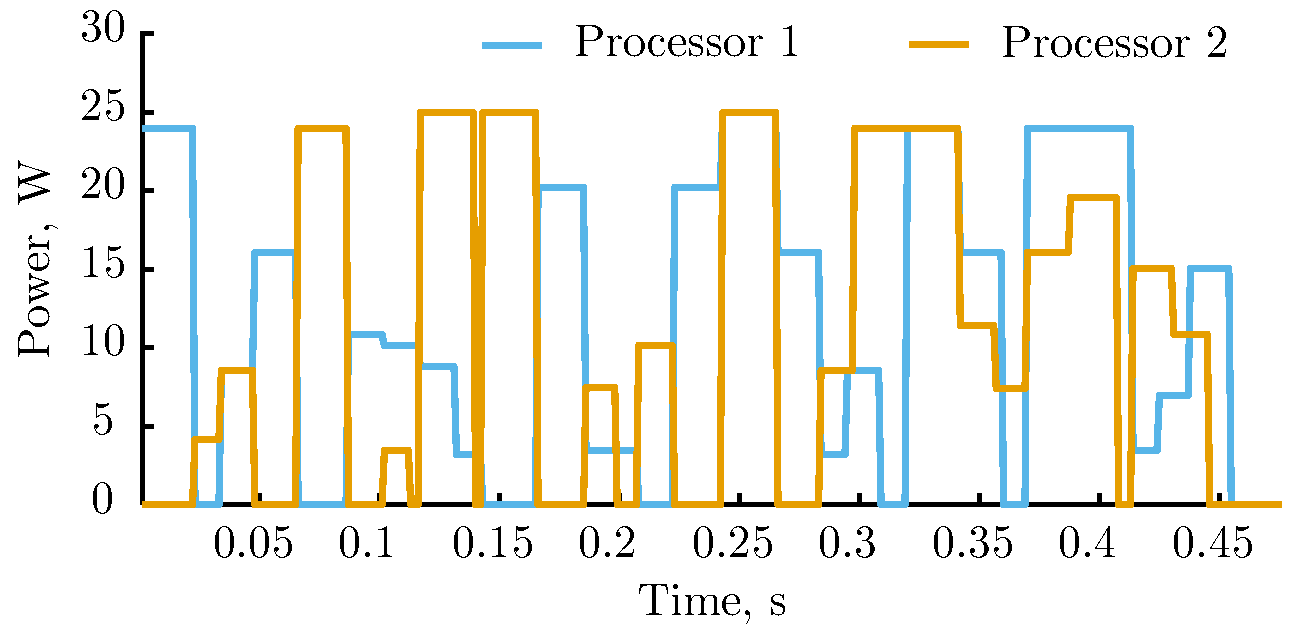
\includegraphics[width=0.90\columnwidth]{include/assets/power.pdf}
  \caption{A dynamic power profile.}
  \flabel{power}
  \vspace{-1.2em}
\end{figure}


\step{5}{Post-processing (\sref{output-processing}).}


\end{document}
